%  LaTeX support: latex@mdpi.com

\documentclass[symmetry,article,submit,pdftex,moreauthors]{Definitions/mdpi}

% MDPI internal commands - do not modify
\firstpage{1}
\makeatletter
\setcounter{page}{\@firstpage}
\makeatother
\pubvolume{1}
\issuenum{1}
\articlenumber{0}
\pubyear{2026}
\copyrightyear{2026}
\datereceived{ }
\daterevised{ }
\dateaccepted{ }
\datepublished{ }

\Title{Multi-Granularity Feature Decomposition with Ranking-Aware Regularization for Old Film Restoration}

% Author information for MGFROFR paper
% MDPI Symmetry format
% This file is input by MGFROFR.tex.

\newcommand{\orcidauthorA}{0009-0000-1111-7667}
\newcommand{\orcidauthorB}{0000-0002-3827-1522}

\Author{Feifan Cai $^{1,2,3}$\orcidA{}, Qi Zhang $^{1,2}$\orcidB{}, Kun Yang $^{3}$, Lei Chen $^{3}$ and Youdong Ding $^{1,2,}$*}

\AuthorNames{Feifan Cai, Qi Zhang, Kun Yang, Lei Chen and Youdong Ding}

\address{%
$^{1}$ \quad Shanghai Film Academy, Shanghai University, 788 Guangzhong Road, Shanghai 200072, China\\
$^{2}$ \quad Shanghai Engineering Research Center of Motion Picture Special Effects, Shanghai 200072, China\\
$^{3}$ \quad College of Mechanical Engineering, Taiyuan University of Technology, Taiyuan 030024, China}

\corres{Correspondence: ydding@shu.edu.cn (Y.D.)}

\abstract{Old film restoration remains difficult because archival footage often contains scratches, blotches, flicker, blur, and temporal artifacts that act at different spatial and temporal scales. These mixed degradations make structural recovery, regional texture repair, and fine artifact suppression compete within a restoration model. We propose MgfrOFR, a multi-granularity extension of a Mamba-based old film restoration backbone. MgfrOFR decomposes propagated features into coarse-to-fine restoration branches and feeds branch summaries back through channel-wise recalibration, so that different degradation scales can be represented without relying on a single feature stream. It also introduces a ranking-aware triplet regularizer that penalizes correlated temporal-similarity rankings across branches during training while preserving the baseline inference interface. Experiments on the SRWOV benchmark show statistically significant PSNR and SSIM gains on synthetic clips, the best NIQE and BRISQUE scores among the compared methods on real-world archival footage, and competitive CLIP-IQA+. These results support the narrower claim that balancing coarse-to-fine feature branches with ranking-aware regularization improves old film restoration under heterogeneous degradation.}


\keyword{old film restoration; multi-granularity feature decomposition; ranking-aware regularization; state space models; feature-space symmetry}

\usepackage{algorithm}
\usepackage{algpseudocode}
\usepackage{placeins}
\renewcommand{\topfraction}{0.9}
\renewcommand{\bottomfraction}{0.8}
\renewcommand{\textfraction}{0.08}
\renewcommand{\floatpagefraction}{0.85}
\setlength{\textfloatsep}{10pt plus 2pt minus 2pt}
\setlength{\floatsep}{8pt plus 2pt minus 2pt}
\setlength{\intextsep}{8pt plus 2pt minus 2pt}
\setlength{\headheight}{20pt}

% Reduce widow/orphan penalties to prevent large blank areas caused by
% MDPI's strict default (10000). 300 still discourages widows/clubs
% but allows LaTeX to break paragraphs when a page has remaining space.
\clubpenalty=300
\widowpenalty=300
\displaywidowpenalty=300

% On float pages (pages that contain only floats), LaTeX vertically centers
% the content by default. Set top/bottom glue to 0 so floats stack at the
% top, eliminating the large blank areas above figures on dedicated float pages.
\makeatletter
\setlength{\@fptop}{0pt}
\setlength{\@fpbot}{0pt}
\makeatother

\AtBeginDocument{\hypersetup{
  pdftitle={Multi-Granularity Feature Decomposition with Ranking-Aware Regularization for Old Film Restoration},
  pdfsubject={Representation-level symmetry-aware multi-granularity feature balancing for old film restoration},
  pdfauthor={Feifan Cai; Qi Zhang; Kun Yang; Lei Chen; Youdong Ding},
  pdfkeywords={old film restoration, symmetry-aware representation learning, multi-granularity features, state space model}
}}

\begin{document}

\section{Introduction}
\label{sec:introduction}

Old film restoration must recover visual content from footage affected by multiple interacting degradation types. Archival film stock often contains scratches, dust, blotches, flicker, blur, grain, and fading within the same clip, and these defects continue to accumulate as the original material deteriorates over time. Digital restoration therefore plays an important role in preserving cinematic heritage, historical documentaries, and large archival collections~\cite{iizuka2019deepremaster}. The technical difficulty is that these degradations occupy different spatial and temporal scales: large missing regions require global context, mid-scale stains require regional repair, and thin scratches or dust require local precision. In this paper, symmetry is used in a limited representation-level sense: the restoration model should keep coarse structural recovery, regional texture repair, and fine artifact suppression balanced even when the observed damage is heterogeneous and asymmetric.

Learning-based old film restoration (OFR) has improved substantially, but existing propagation pipelines still tend to mix different restoration cues in one latent stream. RTN introduced bidirectional recurrent propagation with learnable defect masking~\cite{wan2022rtn}, and RRTN strengthened alignment with recursive transformer propagation~\cite{lin2024rrtn}. MambaOFR adopted state space models for OFR, improved efficiency, and established the SRWOV benchmark~\cite{mao2025mambaofr,gu2024mamba,guo2024mambair}. These methods provide strong temporal modeling, yet structural recovery and fine artifact suppression remain jointly encoded in propagated features. When heterogeneous cues compete in one latent representation, coarse repair can overwrite fine evidence, while aggressive local artifact suppression can distort global structure.

The gap addressed in this work is the absence of an OFR-specific mechanism that separates restoration evidence by granularity and keeps the resulting branches complementary. Multi-granularity designs have been effective in detection and recognition~\cite{lin2017fpn,wang2021hrnet,sun2018pcb,wang2018mgn,gu2025reidmamba}, but those settings use different supervision and feature semantics. A direct multi-branch extension for OFR may also collapse into correlated branches unless diversity is explicitly regularized. Old film restoration therefore requires both a coarse-to-fine decomposition of propagated restoration features and a training signal that discourages redundant branch behavior.

To address this limitation, we propose MgfrOFR, which augments MambaOFR with a Multi-Granularity Feature Extractor (MGFE) and Ranking-Aware Triplet Regularization (RATR). MGFE reorganizes propagated Mamba features into coarse-to-fine restoration branches, allowing structural completion, regional repair, and fine-detail suppression to be represented by dedicated descriptors rather than a single hidden stream. RATR further penalizes correlated temporal-similarity rankings across branches during training, reducing redundant branch behavior without changing the baseline inference interface. Under a unified reproduction protocol on SRWOV, MgfrOFR retains the efficient MambaOFR backbone while adding explicit granularity control with modest overhead. The main contributions are summarized as follows:
\begin{enumerate}
    \item We formulate old film restoration from a restrained representation-level symmetry perspective. The formulation treats coarse structural recovery, regional texture repair, and fine artifact suppression as complementary feature components that should remain balanced under degradation-induced spatial and temporal asymmetry.
    \item We design a multi-granularity feature decomposition mechanism for Mamba-based old film restoration. MGFE inserts learnable restoration tokens into propagated features, progressively aggregates them into coarse-to-fine branches, and feeds branch summaries back to the spatial stream through channel-wise recalibration.
    \item We introduce a ranking-aware triplet regularizer to improve branch complementarity during training. By penalizing correlated temporal-similarity rankings across granularity branches with differentiable rank correlation, RATR reduces redundant branch behavior while preserving the original baseline inference interface.
    \item We conduct a unified evaluation on the SRWOV benchmark covering synthetic and real-world archival footage. The results, statistical tests, ablation studies, and complexity analysis show that MgfrOFR improves restoration fidelity and no-reference naturalness with modest additional computational cost.
\end{enumerate}

\section{Related Work}
\label{sec:related}

\subsection{Old Film and Video Restoration}
\label{subsec:ofr}

Old film restoration differs from general video restoration because it must jointly address structured artifacts, photometric degradation, and quality degeneration. Scratches, dust, and blotches require defect-aware repair, while flicker, grain, fading, blur, and noise require photometric and temporal correction. Traditional approaches decompose the problem into detection and inpainting stages, using hand-crafted features with interpolation-based filling~\cite{kokaram2004missing} or sparse collaborative filtering~\cite{dabov2007bm3d,he2013guided}. Deep learning shifted OFR toward end-to-end restoration: DeepRemaster~\cite{iizuka2019deepremaster} processes spatiotemporal volumes with 3D convolutions, RTN~\cite{wan2022rtn} introduces bidirectional recurrent propagation with a learnable soft defect mask, RRTN~\cite{lin2024rrtn} strengthens alignment with recursive transformer networks and second-order grid propagation, and MambaOFR~\cite{mao2025mambaofr} uses MambaIR-style~\cite{guo2024mambair} state-space modules while introducing the SRWOV benchmark.

Existing video restoration and enhancement systems provide useful context but are not tailored to OFR-specific defect structure. General video restoration methods such as EDVR~\cite{wang2019edvr}, BasicVSR~\cite{chan2021basicvsr}, BasicVSR++~\cite{chan2022basicvsrpp}, VRT~\cite{liang2024vrt}, and RVRT~\cite{liang2022rvrt} model temporal information effectively, but they do not explicitly handle old-film defects. Diffusion and foundation-prior systems, including DiffBIR~\cite{lin2024diffbir}, SUPIR~\cite{yu2024supir}, and SeeSR~\cite{wu2024seesr}, improve perceptual detail for blind image restoration or real-world super-resolution, but they are not designed around temporal old-film artifacts or SRWOV-style video protocols. This leaves a specific need for propagation features that can separate structural completion, regional repair, and fine artifact suppression.

\subsection{State Space Models for Vision}
\label{subsec:ssm}

State space models offer an efficient alternative to attention-heavy restoration backbones. The computational cost of self-attention scales quadratically with sequence length, which is costly for high-resolution video. Structured state space sequence models~\cite{gu2022s4} reformulate sequence modeling through continuous-time state transitions, reducing complexity from $O(L^2)$ to $O(L)$ while maintaining a global receptive field. Mamba~\cite{gu2024mamba} further introduces selective state transitions with hardware-aware recurrence. In vision, MambaIR~\cite{guo2024mambair} demonstrates 2D selective scanning for image restoration, VMamba~\cite{liu2024vmamba} builds hierarchical feature pyramids with four scanning routes, and VSRM~\cite{tran2025vsrm} alternates spatial and temporal Mamba blocks for video super-resolution at linear cost.

These properties are well suited to OFR, which combines long temporal dependency, large spatial damage, and high-resolution input. MambaOFR~\cite{mao2025mambaofr} shows that Mamba-based propagation can improve both efficiency and restoration quality relative to transformer counterparts. However, long-range aggregation alone does not specify which degradation scale each feature should represent. MgfrOFR therefore augments the SSM feature flow with explicit multi-granularity descriptors rather than replacing the backbone.

\subsection{Multi-Scale and Multi-Branch Representations}
\label{subsec:multigran}

Multi-scale and multi-branch representations are useful when one feature scale cannot capture both global context and fine local evidence. Feature Pyramid Networks~\cite{lin2017fpn} and HRNet~\cite{wang2021hrnet} show the value of explicit multi-scale decomposition for dense prediction, while MIRNet-v2~\cite{zamir2022mirnetv2} shows that complementary multi-scale context can improve low-level reconstruction. In person re-identification, PCB~\cite{sun2018pcb} decomposes features along spatial stripes, MGN~\cite{wang2018mgn} combines global and local branches at different partition granularities, and ReIDMamba~\cite{gu2025reidmamba} adapts this idea to state space models. These studies motivate branch-structured representations, but their objectives and feature semantics target recognition rather than video restoration.

\subsection{Diversity and Ranking Regularization}
\label{subsec:diversity_ranking}

Branch structure is useful only when the branches capture complementary cues rather than correlated copies of the same evidence. Contrastive learning~\cite{chen2020mocov2} provides a general diversity mechanism, but it does not directly regulate pairwise ordering behavior across branches. Two branches may differ in magnitude while ranking all candidate frames in the same order, producing apparent feature diversity but redundant temporal structure. Differentiable Kendall's Tau~\cite{zheng2023diffkendall} enables gradient-based penalization of correlated rankings, which is directly applicable to flow-guided temporal correspondences in OFR.

\subsection{Representation Symmetry in Restoration}
\label{subsec:symmetry_ai}

For this paper, representation symmetry denotes balanced and comparable organization of complementary restoration evidence rather than visible geometric symmetry. A learned representation becomes unbalanced when optimization favors one dominant cue and suppresses other cues needed for restoration. Feature-fusion and correlation-based representation studies show that multi-view or multi-branch features require explicit organization rather than simple concatenation~\cite{yu2021multiview_tensor_fusion,qian2020multiview_matrix_correlation}, while adjacent image-processing studies use attention, detection, or differential-equation priors to organize heterogeneous visual evidence for anomaly detection, object detection, segmentation, and denoising~\cite{cui2024video_anomaly_iqa_attention,yin2024improved_faster_rcnn,tian2020pde_segmentation_denoising}. Feature-wise modulation provides a practical way to inject conditioning signals into image-processing networks~\cite{perez2018film}. This restricted view is relevant to OFR because film damage is uneven across both spatial regions and frames.

MgfrOFR adapts these ideas to restoration rather than recognition. First, branch tokens are inserted into propagated restoration features rather than identity-oriented embeddings. Second, branch summaries are fed back into the restoration stream through channel-wise recalibration, so they affect reconstruction rather than only auxiliary supervision. Third, positives and negatives are defined by temporal correspondence within and across clips rather than person identities. The resulting design addresses two OFR-specific gaps: the lack of explicit multi-granularity decomposition within the temporal propagation pipeline, and the lack of diversity regularization that keeps parallel restoration branches complementary, as detailed in Section~\ref{sec:method}.

\section{Methods}
\label{sec:method}


\begin{figure}[!htbp]
\centering
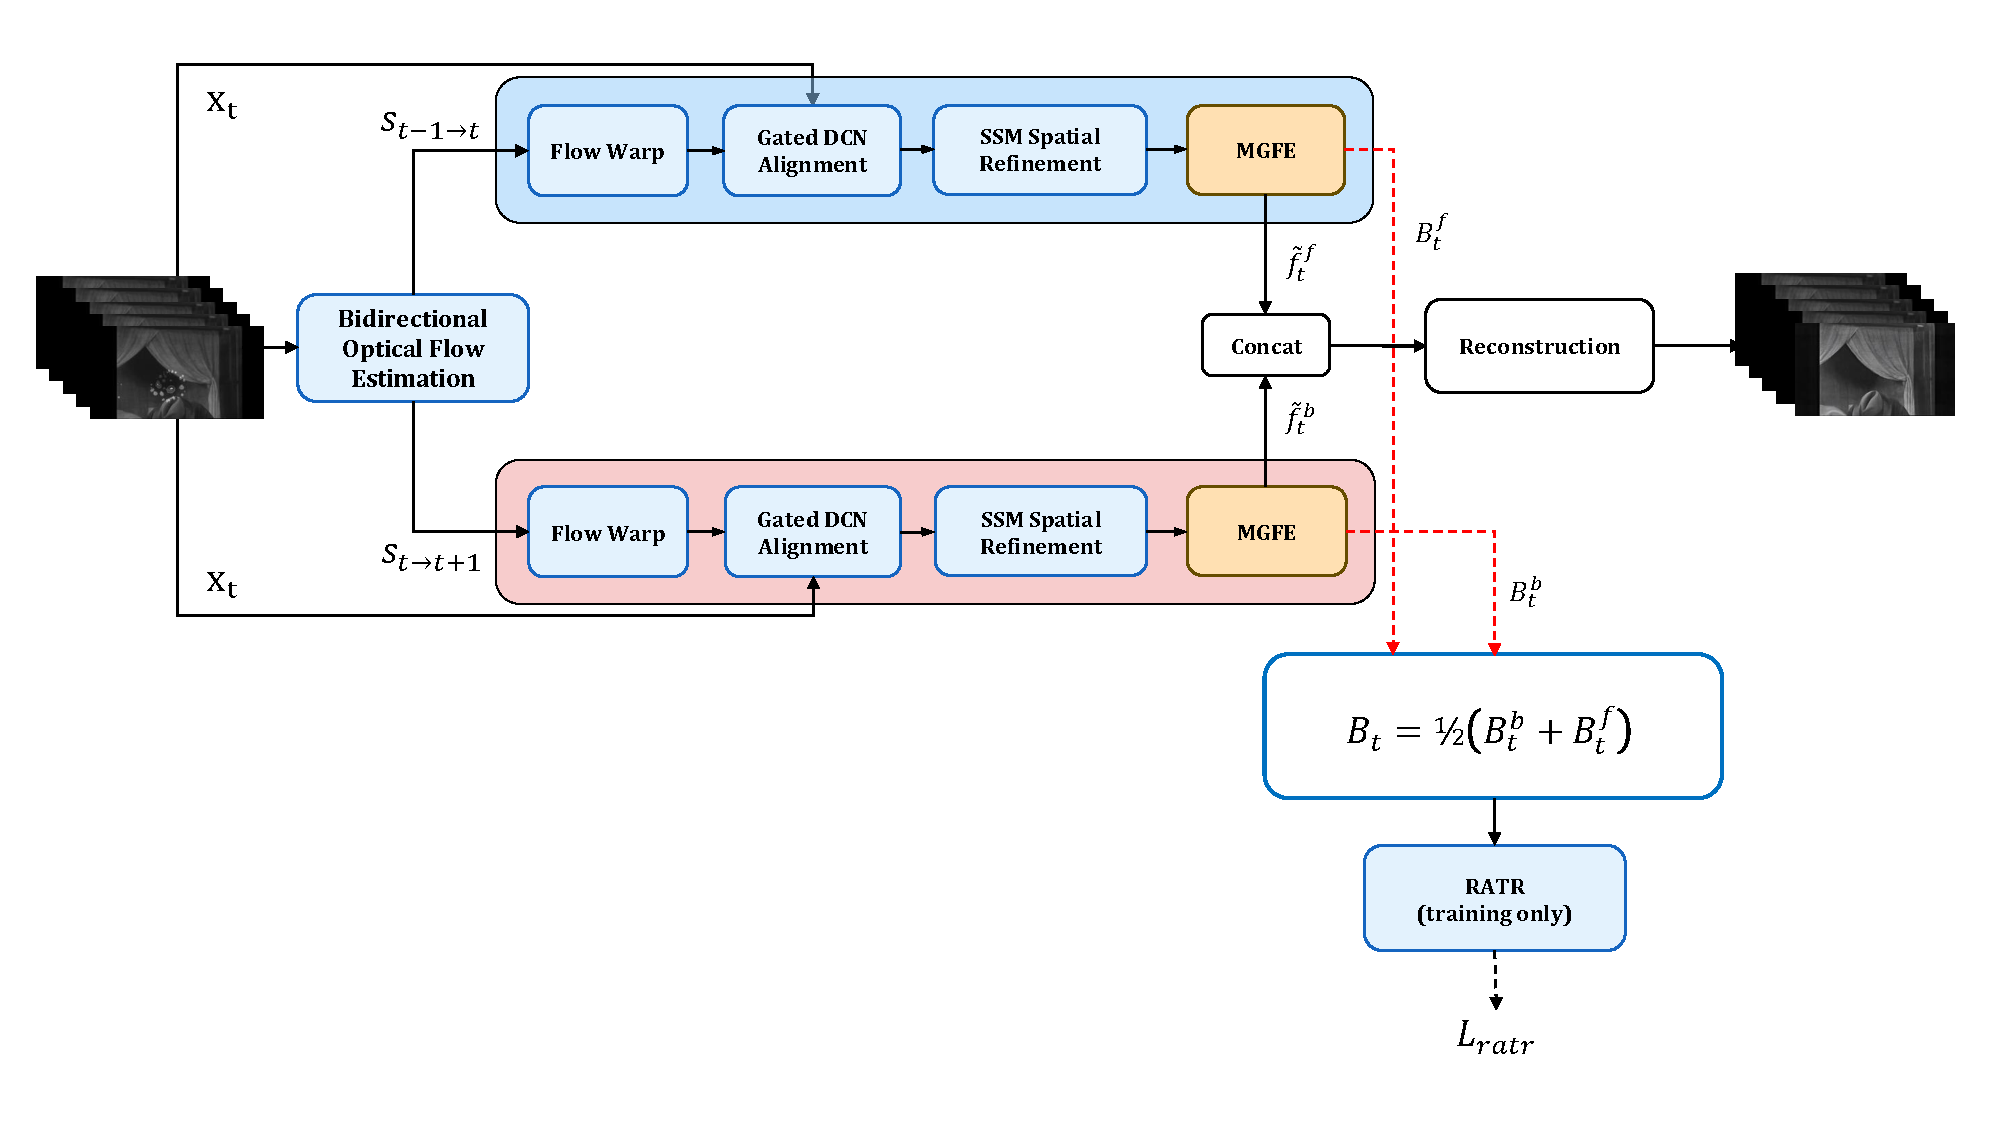
\includegraphics[width=\textwidth]{figures/Fig1_mgfrofr_architecture.pdf}
\caption{MgfrOFR framework. MGFE decomposes propagated features into $G{=}3$ multi-granularity restoration-token branches and uses their summaries for channel-wise recalibration. RATR is used only during training (dashed red path) to penalize redundant temporal-ranking correlations and produce $\mathcal{L}_{\text{intra}}$ and $\mathcal{L}_{\text{inter}}$.\label{fig:architecture}}
\end{figure}

\subsection{Problem Setup}
\label{subsec:problem_setup}

Given a degraded old-film clip $X=\{x_t\}_{t=1}^{T}$, the task is to estimate a restored clip $Y=\{y_t\}_{t=1}^{T}$ that recovers image content while suppressing structured film defects and photometric degradation. Synthetic SRWOV samples provide paired clean frames for direct supervision. Real-world archival clips do not provide ground truth, so their evaluation relies on no-reference quality metrics and qualitative inspection. The method must therefore preserve temporal consistency while handling degradations that vary across both spatial scale and time.

\subsection{Input Representation}
\label{subsec:input_representation}

MgfrOFR operates on the propagated feature maps produced by the baseline bidirectional restoration backbone. For each time step $t$, the backward and forward streams produce aligned feature maps $f_t^{b}, f_t^{f} \in \mathbb{R}^{C_f \times H \times W}$ after motion-aware propagation. MgfrOFR treats these maps as the only interface to the backbone: MGFE reads each propagated map, returns a recalibrated map with the same spatial size and channel count, and emits branch descriptors used by RATR during training.

MgfrOFR follows the same bidirectional propagation framework as MambaOFR~\cite{mao2025mambaofr} while adding an explicit coarse-to-fine representation pipeline. Given a degraded input clip $X=\{x_t\}_{t=1}^{T}$, the baseline first propagates content in backward and forward directions so that neighboring observations are motion-aligned before reconstruction. MgfrOFR then separates restoration evidence by spatial granularity and regularizes the resulting branches during training. In the representation-level symmetry framing used here, coarse, medium, and fine restoration evidence should remain balanced even when the input damage is spatially and temporally asymmetric.

The two added components serve different roles. MGFE converts each propagated feature map into a token sequence, inserts learnable restoration tokens, derives branch descriptors from progressively fused token groups, and feeds their summaries back through channel-wise recalibration. RATR is used only during training; it discourages redundant ranking behavior across branches and does not add an inference module. The reconstruction head follows the original MambaOFR contract and outputs the restored frame. The overall architecture is illustrated in Figure~\ref{fig:architecture}.

\begin{algorithm}[H]
\caption{MgfrOFR forward pass for a clip of length $T$.\label{alg:mgfrofr}}
\begin{algorithmic}[1]
\Require Degraded clip $X=\{x_t\}_{t=1}^{T}$
\Ensure Restored frames $\{y_t\}_{t=1}^{T}$
\State Initialize descriptor buffer $\mathcal{B} \leftarrow \emptyset$
\For{$t = 1$ to $T$}
    \State $f_t^{b}, f_t^{f} \leftarrow \text{Backbone}(X, t)$ \Comment{Bidirectional propagation}
    \For{$d \in \{b, f\}$}
        \State $\widetilde{f}_t^{d}, B_t^{d} \leftarrow \text{MGFE}(f_t^{d})$ \Comment{Multi-granularity decomposition}
    \EndFor
    \State $B_t \leftarrow \frac{1}{2}(B_t^{b} + B_t^{f})$ \Comment{Average branch descriptors}
    \State $\mathcal{B} \leftarrow \mathcal{B} \cup \{B_t\}$ \Comment{Accumulate into batch buffer}
    \State $y_t \leftarrow \mathcal{R}([\widetilde{f}_t^{b}; \widetilde{f}_t^{f}], x_t)$ \Comment{Reconstruction}
\EndFor
\If{training}
    \State $\mathcal{L}_{\text{ratr}} \leftarrow \text{RATR}(\{B_t\}_{t=1}^{T})$ \Comment{Applied on full batch after accumulation}
    \State $\mathcal{L}_{\text{total}} \leftarrow \mathcal{L}_{\text{pix}} + \lambda_{\text{perc}}\mathcal{L}_{\text{perc}} + \lambda_{\text{gan}}\mathcal{L}_{\text{gan}} + \lambda_{\text{ratr}}\mathcal{L}_{\text{ratr}}$
\EndIf
\end{algorithmic}
\end{algorithm}

\subsection{Pipeline Overview}
\label{subsec:overview}

For each time step $t$, the backward and forward propagation paths of the baseline produce feature maps $f_t^{b}, f_t^{f} \in \mathbb{R}^{C_f \times H \times W}$. MGFE transforms each propagated feature into a recalibrated feature map and a set of branch descriptors:

\begin{equation}
\left(\widetilde{f}_t^{d}, B_t^{d}\right)=\operatorname{MGFE}\!\left(f_t^{d}\right), \quad d \in \{b,f\},
\end{equation}

where $d$ indexes the propagation direction, $B_t^{d} \in \mathbb{R}^{G \times D}$ is the branch-descriptor tensor and $D=C_f$ in this work. The reconstruction head keeps the original MambaOFR interface and combines the two recalibrated directional features:

\begin{equation}
y_t = \mathcal{R}\!\left([\widetilde{f}_t^{b};\widetilde{f}_t^{f}], x_t\right),
\qquad
B_t = \frac{1}{2}\left(B_t^{b}+B_t^{f}\right),
\label{eq:mgfrofr_overview_2}
\end{equation}

where $\mathcal{R}(\cdot)$ denotes the unchanged reconstruction head of MambaOFR and $[\cdot;\cdot]$ denotes channel concatenation. Equation~\eqref{eq:mgfrofr_overview_2} matches the implemented data flow: the directional descriptors are averaged before RATR is applied, so the diversity constraint acts on one descriptor tensor per frame rather than duplicating a similar constraint on two directional streams. Figure~\ref{fig:architecture} illustrates the same data flow, and Algorithm~\ref{alg:mgfrofr} summarizes the forward pass.

\subsection{Baseline Interface and Preserved Components}
\label{subsec:baseline_interface}

MgfrOFR preserves the MambaOFR backbone, bidirectional propagation order, reconstruction head, and training loop. The only inference-time insertion is MGFE, which maps $f_t^{d}$ to $\widetilde{f}_t^{d}$ without changing tensor shape. RATR is an auxiliary training loss over branch descriptors and is disabled during inference. This interface keeps the baseline reconstruction contract unchanged: the head still receives concatenated backward and forward propagated features together with the current degraded frame.

\subsection{Multi-Granularity Feature Extractor (MGFE)}
\label{subsec:mgfe}

MGFE separates restoration evidence by spatial granularity while keeping the propagated feature map as the spatial carrier for reconstruction. Large missing regions, mid-scale blotches, and thin scratches require different aggregation ranges, but a single hidden tensor does not require these cues to remain separable. MGFE addresses this by exposing multiple restoration-token branches with different aggregation rates and feeding their summaries back as a recalibration signal. This component provides the branch-balance mechanism of MgfrOFR: each degradation scale receives a dedicated descriptor while reconstruction still uses a common spatial feature carrier. Figure~\ref{fig:mgfe_detail} shows the detailed design.

\begin{figure}[!htbp]
\centering
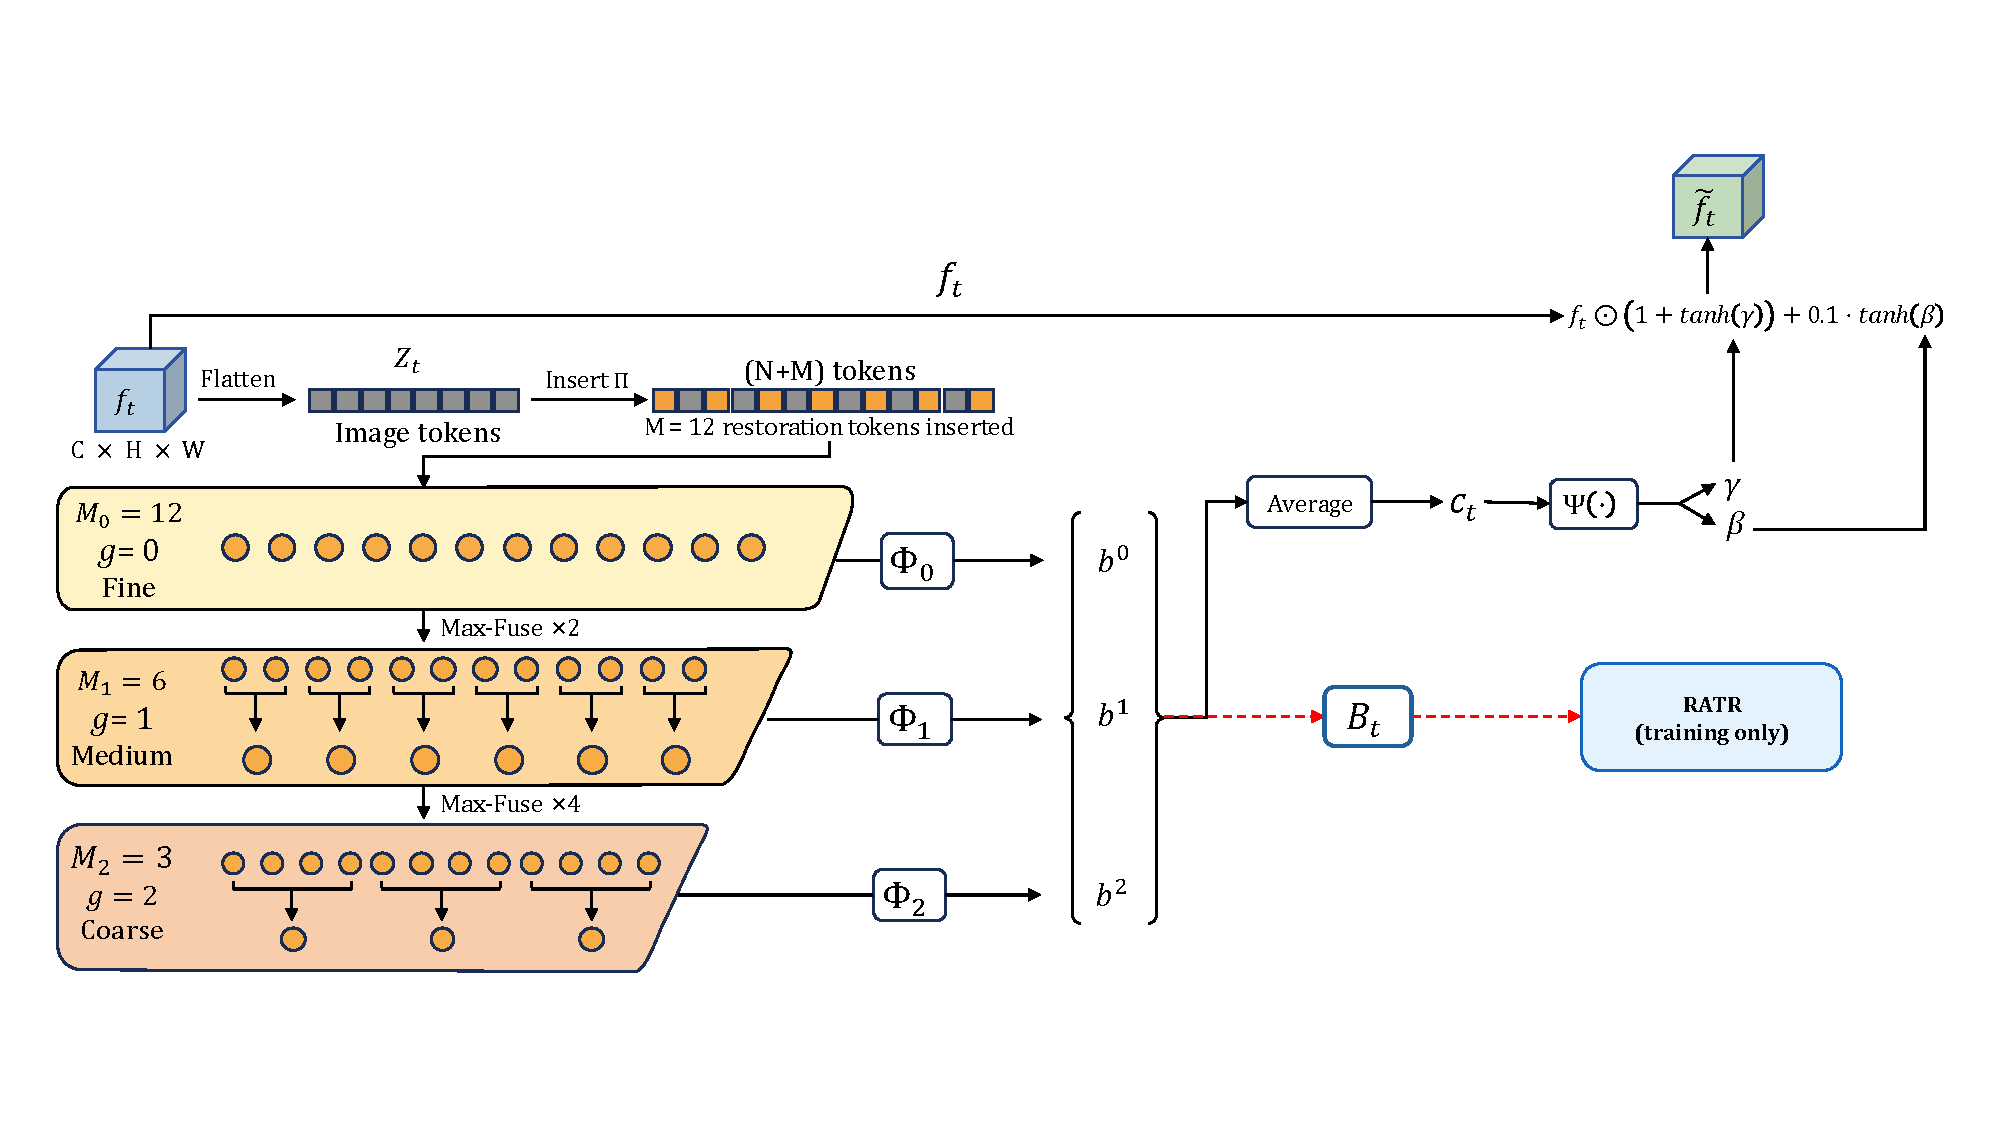
\includegraphics[width=\textwidth]{figures/Fig2_mgfe_module_detail.pdf}
\caption{MGFE module. $M{=}12$ learnable restoration tokens are inserted into image tokens, fused by progressive max fusion, and summarized into $G{=}3$ restoration-token branches. The resulting descriptors generate scale and shift parameters for channel-wise recalibration.\label{fig:mgfe_detail}}
\end{figure}

Since MGFE processes each propagation direction identically, we drop the direction superscript $d$ and write $f_t \in \mathbb{R}^{C_f \times H \times W}$ for brevity. We first flatten it into an image-token sequence

\begin{equation}
Z_t = \operatorname{Flat}(f_t) \in \mathbb{R}^{N \times C_f},
\qquad
N = H W,
\end{equation}

where $\operatorname{Flat}(\cdot)$ preserves raster order and stacks spatial positions into token form. We then append $M$ learnable restoration tokens $R \in \mathbb{R}^{M \times C_f}$ and insert them into the image-token stream through an operator $\Pi(\cdot,\cdot)$:

\begin{equation}
\widehat{Z}_t = \Pi(Z_t, R) \in \mathbb{R}^{(N+M)\times C_f}.
\end{equation}

The insertion operator $\Pi$ distributes restoration tokens uniformly across the image-token stream. It partitions the $N$ image tokens into $M{+}1$ approximately equal chunks and places one restoration token after each of the first $M$ chunks while preserving raster order. Each chunk receives $\lfloor N/(M{+}1)\rfloor$ or $\lceil N/(M{+}1)\rceil$ image tokens so that the total remains exactly $N$. For example, with $M=3$ and $N=9$, the four chunks contain $\{3,2,2,2\}$ image tokens, and the three restoration tokens are inserted at cumulative positions $\{3,6,9\}$ within the 12-token interleaved sequence. This deterministic interleaving gives restoration tokens balanced coverage over the full spatial support.

MGFE builds $G$ granularity branches by progressively fusing restoration tokens. The fusion scheme follows ReIDMamba~\cite{gu2025reidmamba} and is adapted here to propagated spatial restoration features. To make every branch well defined, the number of restoration tokens must satisfy the divisibility constraint
\begin{equation}
M = k \cdot 2^{G-1},\quad k \in \mathbb{N}^{+},
\end{equation}
so that every branch size $M_g = M/2^g$ is an integer for $g\in\{0,\ldots,G-1\}$. We use $G=3$ and $M=12$ ($k=3$) throughout; see Section~\ref{subsec:sensitivity} for alternative configurations.

For branch $g \in \{0,\ldots,G-1\}$, MGFE fuses restoration tokens with a sampling rate of $2^g$. The fused restoration tokens are defined as

\begin{equation}
R^{(g)}[j] =
\mathcal{F}\!\left(
\left\{R[j{\cdot}2^g+k]\right\}_{k=0}^{2^g-1}
\right),\quad
j = 0,\ldots,M_g-1,
\end{equation}

where $\mathcal{F}(\cdot)$ denotes an element-wise maximum operator over all tokens in the fusion group:

\begin{equation}
\mathcal{F}\!\left(
\left\{R[j\cdot2^g+k]\right\}_{k=0}^{2^g-1}
\right)
= \max_{0\le k < 2^g}\,R[j\cdot2^g+k]\;\in\mathbb{R}^{C_f}.
\label{eq:max_fusion}
\end{equation}

The max operation is taken channel-wise. We choose max fusion rather than mean fusion because restoration tokens are intended to retain salient degradation evidence such as scratches, cracks, and blotch boundaries. Mean fusion can dilute sparse high-contrast activations within a group, whereas max fusion preserves the strongest activation in each channel. This design follows ReIDMamba~\cite{gu2025reidmamba}, which reports that max fusion outperforms mean fusion for progressive token aggregation in multi-granularity architectures. Smaller $g$ values preserve more tokens and retain finer local detail, while larger $g$ values compress wider support and emphasize coarse restoration context.

The fused tokens are re-inserted into the same image-token sequence using the same uniform-spacing insertion rule:

\begin{equation}
\widehat{Z}_t^{(g)} = \Pi\!\left(Z_t,R^{(g)}\right),
\end{equation}

and the resulting sequence is processed by a lightweight branch-specific token mixer $\Phi_g(\cdot)$:

\begin{equation}
U_t^{(g)} = \Phi_g\!\left(\widehat{Z}_t^{(g)}\right)
\in \mathbb{R}^{(N+M_g)\times C_f},
\end{equation}

where $M_g = M/2^g$. Each $\Phi_g$ consists of two sequential linear-complexity token blocks. Each block contains a context-augmented projection sublayer and a feed-forward sublayer. The projection sublayer applies LayerNorm, computes a global context vector by mean pooling over the token dimension, adds the projected context to the per-token linear projection, and applies a residual connection. The feed-forward sublayer applies LayerNorm followed by a two-layer MLP with GELU activation and hidden dimension $2C_f$, again with a residual connection. Formally, for input tokens $\mathbf{h}$, each block computes
\begin{equation}
\mathbf{h}' = \mathbf{h} + W_t\,\mathrm{LN}(\mathbf{h}) + W_c\,\overline{\mathrm{LN}(\mathbf{h})},\qquad
\mathbf{h}'' = \mathbf{h}' + \mathrm{MLP}(\mathrm{LN}(\mathbf{h}')),
\end{equation}
where $\overline{(\cdot)}$ denotes mean pooling over the token dimension, $W_t,W_c\in\mathbb{R}^{C_f\times C_f}$ are learned projections, and MLP consists of $\mathrm{Linear}(C_f\!\rightarrow\!2C_f)\!\rightarrow\!\mathrm{GELU}\!\rightarrow\!\mathrm{Linear}(2C_f\!\rightarrow\!C_f)$. The global context term $W_c\,\overline{\mathrm{LN}(\mathbf{h})}$ gives each token a lightweight full-sequence summary at linear cost, avoiding the quadratic complexity of self-attention while retaining inter-token communication. Each branch has its own pair of token blocks, allowing branch-specific parameterization with modest overhead.

After branch processing, MGFE summarizes each branch by averaging the updated restoration-token positions:

\begin{equation}
b_t^{(g)} =
\frac{1}{M_g}
\sum_{m=1}^{M_g}
U_t^{(g)}[\pi_m^{(M_g)}]
\in \mathbb{R}^{D},
\end{equation}

where $\{\pi_m^{(M_g)}\}_{m=1}^{M_g}$ denote the uniformly spaced insertion positions for $M_g$ tokens, and $D=C_f$. Stacking all branch descriptors gives

\begin{equation}
B_t =
\left[
b_t^{(0)}, b_t^{(1)}, \ldots, b_t^{(G-1)}
\right]^\top
\in \mathbb{R}^{G \times D}.
\end{equation}

Because the descriptors are extracted from a common propagated feature under different token-fusion rates, they share semantic alignment while differing in granularity. This descriptor tensor $B_t$ is the input to RATR.

MGFE also converts the branch descriptors into a channel-wise recalibration signal. We first average the branch context,

\begin{equation}
c_t = \frac{1}{G}\sum_{g=0}^{G-1}b_t^{(g)},
\qquad
[\boldsymbol{\gamma}_t,\boldsymbol{\beta}_t] = \Psi(c_t),
\label{eq:recalibration_context}
\end{equation}

where $\Psi(\cdot)$ is a projection head consisting of $\mathrm{LayerNorm}\!\rightarrow\!\mathrm{Linear}(C_f\!\rightarrow\!2C_f)\!\rightarrow\!\mathrm{GELU}\!\rightarrow\!\mathrm{Linear}(2C_f\!\rightarrow\!2C_f)$ that outputs concatenated scale and shift vectors. The recalibrated propagated feature is then

\begin{equation}
\widetilde{f}_t =
f_t \odot
\left(1+\tanh(\boldsymbol{\gamma}_t)\right)
+ 0.1\,\tanh(\boldsymbol{\beta}_t),
\label{eq:recalibration}
\end{equation}

where the vectors in Equation~\eqref{eq:recalibration_context} are broadcast over spatial dimensions. The multiplicative term $(1+\tanh(\boldsymbol{\gamma}_t))$ keeps scaling close to unity at initialization, and the additive coefficient $0.1$ limits the shift magnitude. The shift coefficient $0.1$ bounds the additive term to at most $10\%$ of the $\tanh$ range, keeping the modulation within a conservative $10\%$ shift scale. This conservative FiLM-style modulation~\cite{perez2018film} helps the recalibrated feature remain close to the original propagated feature when the branch context is uncertain. Once the branch descriptors become informative, coarse branches can supply global structural preferences and fine branches can emphasize localized damage patterns.

In summary, MGFE separates restoration evidence by spatial granularity through lightweight token mixing while preserving the baseline interface through residual-style recalibration. The branch descriptors $B_t$ and the recalibration signal $(\boldsymbol{\gamma}_t, \boldsymbol{\beta}_t)$ serve two different roles: the descriptors provide ranking targets for RATR (Section~\ref{subsec:ratr}), while the recalibration feeds granularity-aware modulation back into the propagated feature. This separation allows ablation studies to disable recalibration while keeping branch descriptors active for diversity regularization (see the RATR-only configuration in Section~\ref{subsec:ablation}). Explicit branches alone, however, do not guarantee complementary features. If all branches induce the same sample rankings, branch balance degenerates into redundant descriptors. This motivates the training regularizer described next.

\subsection{Ranking-Aware Triplet Regularization (RATR)}
\label{subsec:ratr}

RATR discourages branch collapse by penalizing excessive ranking correlation between branches. A simple diversity loss could force descriptors to be orthogonal, but orthogonality does not ensure that branches organize restoration evidence differently across samples. The relevant behavior is the branch-specific similarity order induced when an anchor frame is compared with nearby positives and harder negatives. If different branches rank the same candidates identically, they remain redundant even if their descriptor values differ. RATR therefore formulates diversity as an anchor-centered ranking problem using Kendall's~\cite{kendall1938measure} rank correlation coefficient, made differentiable by DiffKendall~\cite{zheng2023diffkendall}. Figure~\ref{fig:ratr_detail} illustrates the workflow.

\begin{figure}[!htbp]
\centering
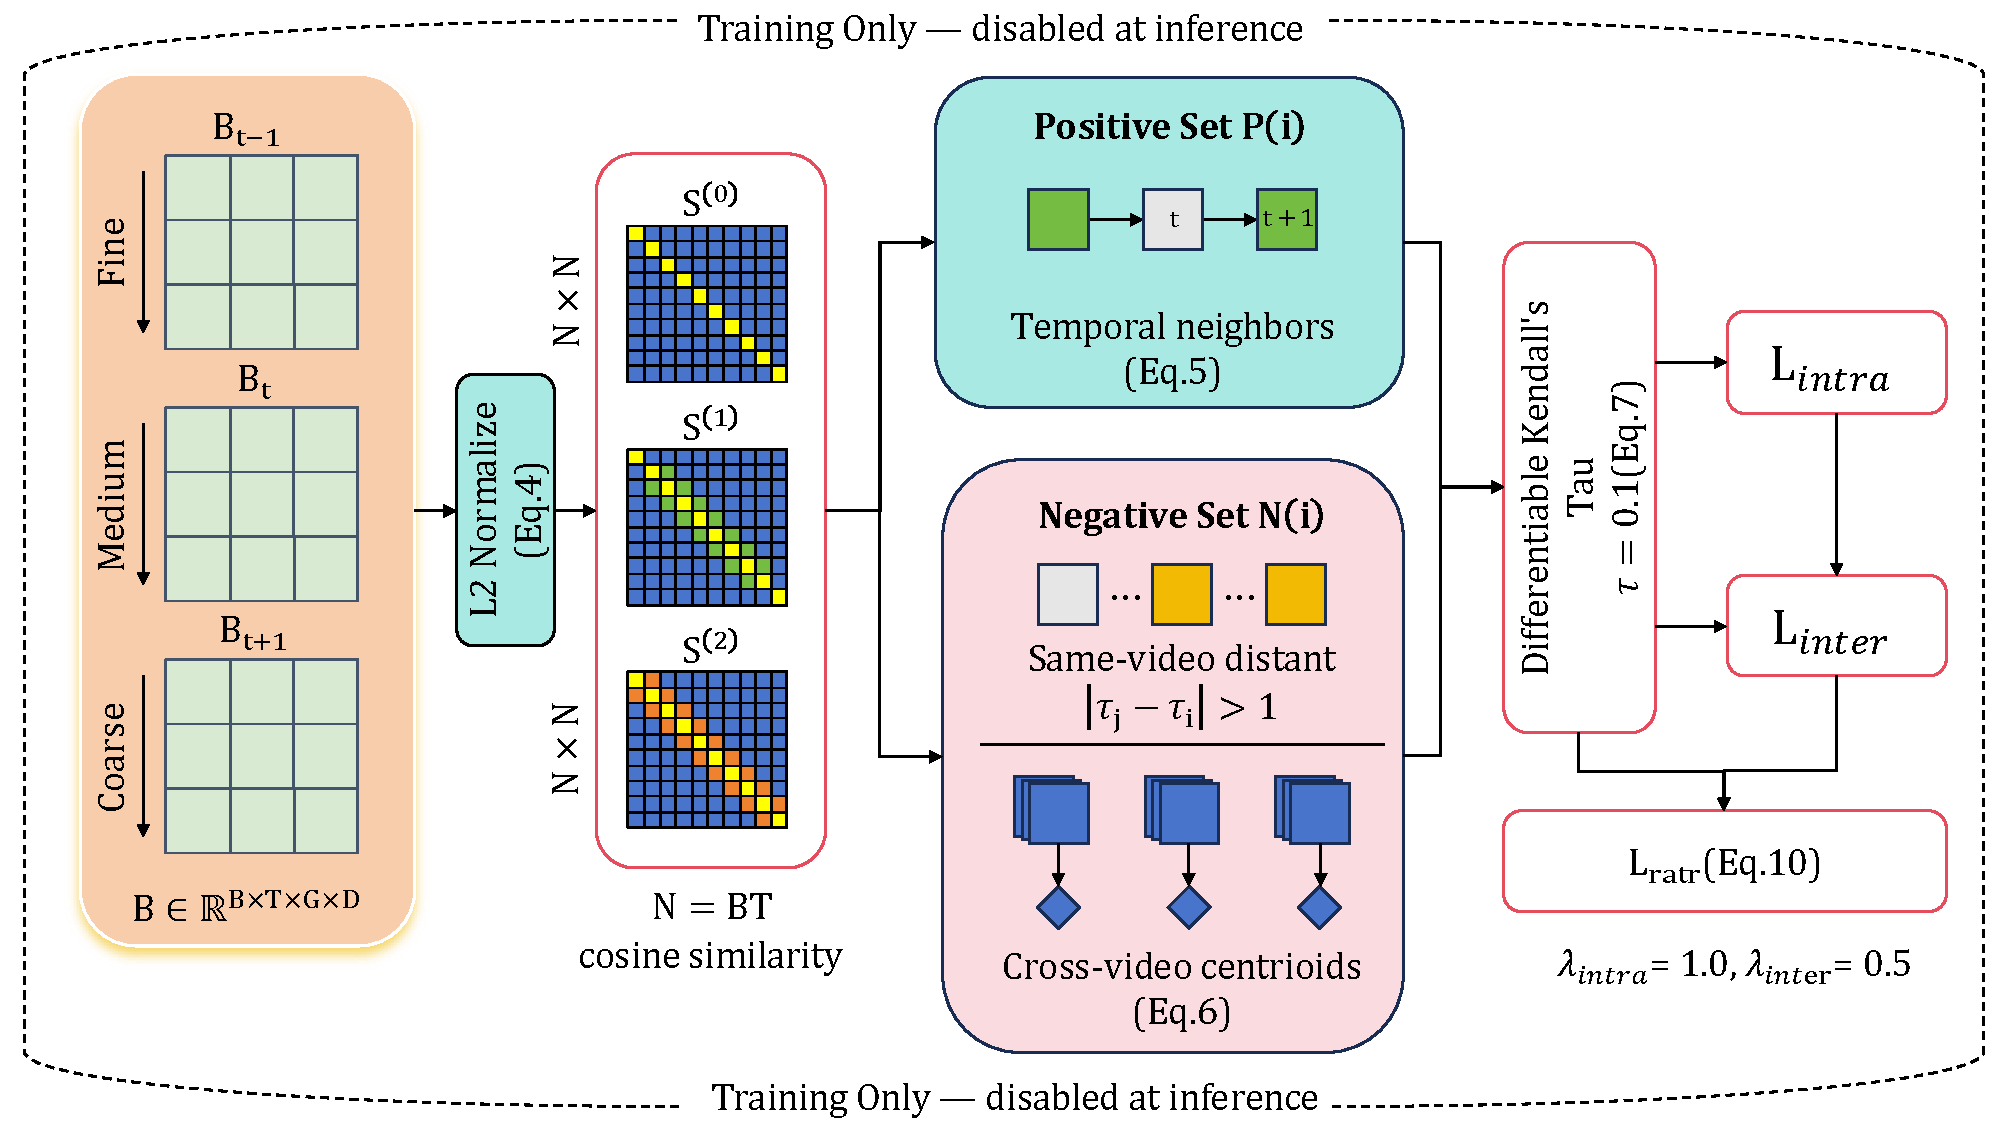
\includegraphics[width=\textwidth]{figures/Fig3_ratr_module_detail.pdf}
\caption{RATR module. Differentiable Kendall's Tau compares branch-specific ranking sequences from temporal correspondences. Neighbor frames define positives, while distant same-video frames and cross-video centroids define negatives, producing $\mathcal{L}_{\text{intra}}$ and $\mathcal{L}_{\text{inter}}$ during training only.\label{fig:ratr_detail}}
\end{figure}

Let the averaged branch descriptors from Equation~\eqref{eq:mgfrofr_overview_2} be organized as a 4D tensor of shape $N_b\times T\times G\times D$, where $N_b$ is the batch size. We flatten batch and time into $\bar{N}=N_b T$ samples and normalize the descriptors branch-wise:

\begin{equation}
\widehat{b}_i^{(g)} =
\frac{b_i^{(g)}}{\|b_i^{(g)}\|_2},
\qquad
i=1,\ldots,\bar{N}.
\end{equation}

For each branch $g$, we compute a cosine-similarity matrix

\begin{equation}
\mathcal{S}^{(g)}[i,j] =
\left\langle
\widehat{b}_i^{(g)},
\widehat{b}_j^{(g)}
\right\rangle.
\end{equation}

This matrix is not used as a standalone supervision target. Instead, it provides the positive and negative ranking sequences that form the anchor-positive-negative structure regularized by RATR.

For anchor $i$, the positive set is defined from temporal correspondences within the same clip:

\begin{equation}
\mathcal{P}(i)=
\bigl\{
j \mid v_j=v_i,\;
|t_j-t_i|=1
\bigr\},
\end{equation}

where $v_i$ and $t_i$ denote the clip index and frame index of sample $i$. This temporal adjacency criterion is justified because the flow-guided deformable alignment in MambaOFR has already warped neighboring frames toward the anchor frame before MGFE is applied. After this alignment, adjacent frames are the most reliable proxy for true flow-based correspondences in the feature domain. Since $|\mathcal{P}(i)| \le 2$, boundary frames provide only one positive neighbor. We therefore evaluate the intra-ranking term only on anchors with at least two positives:
\begin{equation}
\mathcal{I}_{\text{intra}}=
\bigl\{
i \mid |\mathcal{P}(i)| \ge 2
\bigr\}.
\end{equation}
For the seven-frame clips used in training, this excludes only the first and last frame of each clip. Interior anchors then contribute exactly one pairwise ordering comparison to $\mathcal{L}_{\text{intra}}$. This limited signal is sufficient in practice because (i)~$\mathcal{L}_{\text{intra}}$ is averaged over many valid anchors in each batch, and (ii)~$\mathcal{L}_{\text{inter}}$ supplies a complementary ranking signal from the richer negative set.

Negative evidence is drawn from two harder sources: temporally distant frames inside the same clip and clip-level representatives from other clips. The same-video negatives are

\begin{equation}
\mathcal{N}_{sv}(i)=
\bigl\{
j \mid v_j=v_i,\;
|t_j-t_i|>1
\bigr\},
\end{equation}

and the clip-level centroid for another video $v\neq v_i$ is

\begin{equation}
\bar{b}_{v}^{(g)} =
\frac{1}{|\mathcal{T}_v|}
\sum_{t\in\mathcal{T}_v}
\widehat{b}_{(v,t)}^{(g)},
\end{equation}

where $\mathcal{T}_v$ denotes the set of frame indices in clip $v$. We then construct the negative ranking sequence as

\begin{equation}
\bar{\mathcal{S}}_i^{(g)} =
\Bigl[\mathcal{S}^{(g)}[i,j]\Bigr]_{j\in\mathcal{N}_{sv}(i)}
\oplus
\Bigl[\bigl\langle \widehat{b}_i^{(g)},\,\bar{b}_v^{(g)} \bigr\rangle\Bigr]_{v\neq v_i},
\end{equation}

where $\oplus$ denotes sequence concatenation. Same-video distant frames are hard negatives because they share content and degradation statistics with the anchor but are no longer immediate temporal neighbors. Off-video centroids provide a low-variance clip-level representative that avoids the $O(\bar{N}^2)$ cost of enumerating every cross-clip frame pair while still capturing inter-clip distributional contrast.

To compare how two branches rank the same candidate set, we adopt a differentiable version of Kendall's Tau. For sequences $p,q\in\mathbb{R}^{L}$, the differentiable statistic is

\begin{equation}
\mathrm{DKTau}(p,q;\tau)
= \frac{1}{\binom{L}{2}}
\sum_{1\le u < v \le L}
\tanh\!\!\left(\frac{p_u-p_v}{\tau}\right)
\cdot
\tanh\!\!\left(\frac{q_u-q_v}{\tau}\right),
\label{eq:dktau}
\end{equation}

where $\tau>0$ is a temperature parameter. As $\tau\rightarrow 0$, Equation~\eqref{eq:dktau} approaches the hard sign comparison used in the exact Kendall coefficient; as $\tau$ becomes too large, pairwise order differences are oversmoothed and gradients vanish. We set $\tau=0.1$ (see Section~\ref{subsec:sensitivity} for the sensitivity to this choice). A lower value of $\mathrm{DKTau}(p,q;\tau)$ indicates weaker ranking correlation between branches and therefore stronger branch complementarity.

Using Equation~\eqref{eq:dktau}, we compute the positive-ranking correlation loss as

\begin{equation}
\mathcal{L}_{\text{intra}} =
\frac{1}{|\mathcal{I}_{\text{intra}}| \binom{G}{2}}
\sum_{i\in\mathcal{I}_{\text{intra}}}
\sum_{g < g'}
\mathrm{DKTau}\!\Bigl(
\mathcal{S}^{(g)}[i,\mathcal{P}(i)],\,
\mathcal{S}^{(g')}[i,\mathcal{P}(i)];\,\tau
\Bigr),
\label{eq:loss_intra}
\end{equation}

and the negative-ranking correlation loss as

\begin{equation}
\mathcal{L}_{\text{inter}} =
\frac{1}{\bar{N} \binom{G}{2}}
\sum_{i=1}^{\bar{N}}
\sum_{g < g'}
\mathrm{DKTau}\!\Bigl(
\bar{\mathcal{S}}_i^{(g)},\,
\bar{\mathcal{S}}_i^{(g')};\,
\tau
\Bigr).
\end{equation}

The final ranking-aware regularizer is

\begin{equation}
\mathcal{L}_{\text{ratr}} =
\lambda_{\text{intra}}\,\mathcal{L}_{\text{intra}}
+ \lambda_{\text{inter}}\,\mathcal{L}_{\text{inter}}.
\label{eq:loss_ratr}
\end{equation}

Equations~\eqref{eq:loss_intra}--\eqref{eq:loss_ratr} play complementary roles. The intra term prevents two branches from assigning nearly identical orders to the most likely temporal correspondences, while the inter term prevents the same collapse on harder negatives. Minimizing both terms does not force arbitrary disagreement because the restoration losses still anchor the recalibrated feature stream to the reconstruction target through MGFE.

\subsection{Training Objective}
\label{subsec:training_objective}

The generator objective combines the standard OFR losses used by the MambaOFR baseline with the proposed ranking-aware regularizer. Specifically, we use an $L_1$ pixel reconstruction loss $\mathcal{L}_{\mathrm{pix}}$, whose robustness for image restoration objectives is analyzed in~\cite{zhao2017loss_restoration}, a VGG-based perceptual loss $\mathcal{L}_{\mathrm{perc}}$~\cite{johnson2016perceptual}, an adversarial loss $\mathcal{L}_{\mathrm{gan}}$~\cite{goodfellow2014gan}, and the proposed ranking regularization $\mathcal{L}_{\mathrm{ratr}}$:

\begin{equation}
\mathcal{L}_{\mathrm{total}} =
\mathcal{L}_{\mathrm{pix}}
+ \lambda_{\mathrm{perc}}\mathcal{L}_{\mathrm{perc}}
+ \lambda_{\mathrm{gan}}\mathcal{L}_{\mathrm{gan}}
+ \lambda_{\mathrm{ratr}}\mathcal{L}_{\mathrm{ratr}}.
\label{eq:loss_total}
\end{equation}

Equation~\eqref{eq:loss_total} preserves backward compatibility with the baseline training loop because MGFE only augments the propagated feature stream and RATR appears purely as an auxiliary regularizer. The loss weights are set to $\lambda_{\mathrm{perc}}=1.0$ and $\lambda_{\mathrm{gan}}=0.01$, following RTN~\cite{wan2022rtn} and MambaOFR~\cite{mao2025mambaofr}. For the ranking term, we use $\lambda_{\mathrm{ratr}}=0.1$, $\lambda_{\mathrm{intra}}=1.0$, and $\lambda_{\mathrm{inter}}=0.5$ (see Section~\ref{subsec:sensitivity} for sensitivity to these choices). The smaller weight on $\mathcal{L}_{\text{inter}}$ reflects the coarser ordering signal of clip-centroid negatives. Unless otherwise stated, the full model uses feature dimension $C_f=16$, $G=3$ branches, $M=12$ restoration tokens, channel-wise max fusion in Equation~\eqref{eq:max_fusion}, and a differentiable Kendall temperature of $\tau=0.1$.

\section{Experiment}
\label{sec:experiment}

\subsection{Datasets and Evaluation Metrics}
\label{subsec:datasets_metrics}

\subsubsection{Datasets}
\label{subsec:datasets}

We evaluate MgfrOFR on the SRWOV benchmark introduced with MambaOFR~\cite{mao2025mambaofr}. SRWOV is a dedicated old film restoration benchmark with both synthetic and real-world test sets.

Training uses the REDS training split~\cite{nah2019reds}, which contains 240 video sequences, each with 100 frames at $720 \times 1280$ resolution. Clean REDS frames are degraded on the fly using the synthetic degradation pipeline from MambaOFR. This pipeline simulates scratches, dust, blotches, flicker, and grain to produce paired degraded and clean training samples.

Evaluation uses two SRWOV test settings with different evidence types. The synthetic test set contains 30 clips rendered with the same degradation pipeline on held-out REDS sequences. Each clip consists of 100 frames at $720 \times 1280$ resolution and has paired ground truth, enabling full-reference metrics. The real-world set comprises 216 archival clips from the 1920s to 1960s with authentic mixed degradation and no ground truth; it is evaluated with no-reference quality metrics. Following the original SRWOV protocol~\cite{mao2025mambaofr}, we use all 216 real-world clips, covering indoor portraits, newsreel footage, conversations, and multi-person scenes for a total of 29{,}256 frames.

\subsubsection{Evaluation Metrics}
\label{subsec:eval_metrics}

We use seven metrics to cover pixel fidelity, perceptual similarity, and statistical naturalness. For synthetic evaluation with ground truth, PSNR and SSIM~\cite{wang2004ssim} measure pixel-level fidelity (higher is better), LPIPS~\cite{zhang2018lpips} measures learned perceptual distance (lower is better), and DISTS~\cite{ding2020dists} measures structure-and-texture perceptual similarity (lower is better). For real-world evaluation without ground truth, NIQE~\cite{mittal2012niqe} and BRISQUE~\cite{mittal2012brisque} measure statistical naturalness (lower is better), while CLIP-IQA+~\cite{wang2023clipiqa} uses CLIP~\cite{radford2021clip} visual features with learnable quality-aware prompts (higher is better). The metrics are reported separately when they emphasize different aspects of quality.

\subsection{Implementation Details}
\label{subsec:implementation}

\subsubsection{Training Details}
\label{subsubsec:training_details}

We train MgfrOFR on the REDS training split~\cite{nah2019reds} with the synthetic degradation pipeline described in Section~\ref{subsec:datasets}. Optimization uses Adam~\cite{kingma2015adam} with $\beta_1=0.9$ and $\beta_2=0.99$, an initial learning rate of $2\times10^{-4}$, and a MultiStep scheduler with milestones at 50K, 100K, and 150K iterations ($\gamma=0.5$). Training runs for $200$K iterations on $4$ NVIDIA A100 GPUs (80\,GB each), with one clip per GPU per mini-batch. Each training sample contains $T=7$ consecutive frames cropped to $256\times256$. The software stack consists of PyTorch 2.7 and CUDA 12.4, with the random seed fixed to 42 for reproducibility. At inference, RATR is disabled and frames are processed at full resolution ($720 \times 1280$) without cropping.

\subsubsection{Baseline Adaptation Protocol}
\label{subsubsec:baseline_adaptation}

The comparison uses released implementations and published settings where available, reproduced in a unified environment. Dedicated OFR methods (RTN, RRTN, MambaOFR) are trained or reproduced under the same REDS-based synthetic film pipeline. For generic video restoration methods (VRT, RVRT, ShiftNet), we preserve the published architecture and default optimization recipe while replacing only the task-specific degradation generation so that the methods can be trained on OFR-style inputs. Enhancement-oriented methods (DeOldify, OldPhoto, DeepRemaster) are included as reference systems to contextualize perceptual trade-offs rather than as fully task-matched OFR baselines. We therefore interpret the comparison as a unified reproduction study under a common degradation protocol, not as evidence that every baseline has been exhaustively re-optimized for OFR.

\subsection{Comparison with State-of-the-Art}
\label{subsec:comparison_sota}

We compare MgfrOFR against nine baselines spanning dedicated OFR methods, general video restoration models, and image/video enhancement approaches. The dedicated OFR baselines are RTN~\cite{wan2022rtn}, RRTN~\cite{lin2024rrtn}, and MambaOFR~\cite{mao2025mambaofr}; the general video restoration baselines are VRT~\cite{liang2024vrt}, RVRT~\cite{liang2022rvrt}, and ShiftNet~\cite{li2023shiftnet}; and the enhancement-oriented references are DeOldify~\cite{jantic2019deoldify}, OldPhoto~\cite{wan2023oldphotopami}, and DeepRemaster~\cite{iizuka2019deepremaster}. No-reference metrics are computed using the pyiqa library under the same software environment.

\subsubsection{Quantitative Comparison on Synthetic Data}

Table~\ref{tab:sota} reports full-reference evaluation on the SRWOV synthetic benchmark. MgfrOFR achieves the best PSNR/SSIM and the lowest LPIPS (0.0789) and DISTS (0.0653), surpassing the strongest baseline MambaOFR by +1.14~dB PSNR. The pattern is consistent with the intended architectural distinction: generic video restoration methods do not include OFR-specific defect handling, while frame-oriented enhancement approaches can suffer from temporal inconsistency.

\begin{table}[htbp]
\caption{Quantitative comparison reports SRWOV synthetic full-reference results under the unified reproduction protocol. Best results are in \textbf{bold}, second best are \underline{underlined}.\label{tab:sota}}
\begin{tabularx}{\textwidth}{lCCCC}
\toprule
\textbf{Method} & \textbf{PSNR$\uparrow$} & \textbf{SSIM$\uparrow$} & \textbf{LPIPS$\downarrow$} & \textbf{DISTS$\downarrow$} \\
\midrule
ShiftNet~\cite{li2023shiftnet}          & 21.48 & 0.8234 & 0.2030 & 0.1303 \\
VRT~\cite{liang2024vrt}                 & 22.39 & 0.8631 & 0.1750 & 0.1087 \\
RVRT~\cite{liang2022rvrt}              & 22.43 & 0.8710 & 0.1655 & 0.1078 \\
DeOldify~\cite{jantic2019deoldify}      & 23.22 & 0.8923 & 0.2775 & 0.1260 \\
RRTN~\cite{lin2024rrtn}                & 24.15 & 0.9006 & 0.1082 & \underline{0.0668} \\
OldPhoto~\cite{wan2023oldphotopami}     & 24.62 & 0.8524 & 0.2252 & 0.1144 \\
DeepRemaster~\cite{iizuka2019deepremaster} & 25.06 & \underline{0.9185} & 0.1108 & 0.0895 \\
RTN~\cite{wan2022rtn}                   & 25.85 & 0.8869 & 0.1214 & 0.0862 \\
MambaOFR~\cite{mao2025mambaofr}        & \underline{25.99} & 0.9059 & \underline{0.0815} & 0.0822 \\
\midrule
MgfrOFR (Ours)                          & \textbf{27.13} & \textbf{0.9237} & \textbf{0.0789} & \textbf{0.0653} \\
\bottomrule
\end{tabularx}
\end{table}

To test whether the gain over MambaOFR is clip-consistent, we apply paired, two-sided Wilcoxon signed-rank tests to the 30 per-clip means. MgfrOFR improves PSNR on 29/30 clips ($p=3.7\times10^{-9}$) and SSIM on 23/30 clips ($p=3.5\times10^{-3}$), with a median per-clip $\Delta$PSNR of 1.77~dB and an interquartile range of [1.06, 2.82]~dB; LPIPS ($p=0.71$) and DISTS ($p=0.11$) are not significant at $N{=}30$.

\subsubsection{Quantitative Comparison on Real-World Data}

Table~\ref{tab:realworld} reports no-reference quality metrics on 216 real-world archival clips from the SRWOV real-world set, where ground truth is unavailable. Because NIQE and BRISQUE emphasize statistical naturalness whereas CLIP-IQA+ reflects CLIP-aligned perceptual quality, we report the metrics separately rather than collapsing them into a single aggregate ranking. All methods are evaluated on the full 216-clip set under the same pyiqa-based metric environment.

\begin{table}[htbp]
\caption{Real-world evaluation reports no-reference quality metrics on SRWOV real footage under the same pyiqa-based metric environment.\label{tab:realworld}}
\begin{tabularx}{\textwidth}{lCCC}
\toprule
\textbf{Method} & \textbf{NIQE$\downarrow$} & \textbf{BRISQUE$\downarrow$} & \textbf{CLIP-IQA+$\uparrow$} \\
\midrule
ShiftNet~\cite{li2023shiftnet}             & 5.71  & 42.82 & 0.3975 \\
VRT~\cite{liang2024vrt}                    & 5.66  & 42.73 & 0.3985 \\
RVRT~\cite{liang2022rvrt}                 & 5.72  & 42.64 & 0.4013 \\
DeOldify~\cite{jantic2019deoldify}         & 5.72  & 41.61 & 0.3768 \\
RRTN~\cite{lin2024rrtn}                   & 5.67  & 32.86 & 0.3969 \\
OldPhoto~\cite{wan2023oldphotopami}        & 6.56  & 30.45 & \textbf{0.4503} \\
DeepRemaster~\cite{iizuka2019deepremaster} & 5.99  & 40.62 & 0.3991 \\
RTN~\cite{wan2022rtn}                      & \underline{5.17}  & \underline{19.00} & 0.4163 \\
MambaOFR~\cite{mao2025mambaofr}           & 5.34  & 29.79 & 0.4351 \\
\midrule
MgfrOFR (Ours)                             & \textbf{5.06}  & \textbf{18.70} & \underline{0.4368} \\
\bottomrule
\end{tabularx}
\end{table}

MgfrOFR obtains the best NIQE (5.06) and BRISQUE (18.70) among the compared methods. Relative to the previous best RTN (5.17 / 19.00), the dataset averages improve by $-2.1\%$ on NIQE and $-1.6\%$ on BRISQUE, indicating better statistical naturalness under these no-reference metrics. MgfrOFR also attains competitive CLIP-IQA+ (0.4368), ranking second to OldPhoto (0.4503) and ahead of MambaOFR (0.4351). Because the three no-reference metrics quantify different perceptual attributes, these results should not be collapsed into a single superiority claim. The gap to OldPhoto on CLIP-IQA+ is discussed in Section~\ref{subsec:failure}.

\subsubsection{Qualitative Comparison}

\begin{figure}[htbp]
\centering
\includegraphics[width=0.95\textwidth]{figures/Fig4_SOTA_Synthetic_REDS_synthetic_Qualitative_roi_tile_special.jpg}
\caption{Qualitative comparison on four representative SRWOV synthetic scenes. Columns (a)--(l) show the degraded input, DeOldify, ShiftNet, VRT, RVRT, OldPhoto, DeepRemaster, RTN, RRTN, MambaOFR, MgfrOFR (Ours), and the ground truth. Red and green boxes mark local regions in each overview row, and the ROI tiles below each row enlarge the corresponding damaged structures. The comparison illustrates that MgfrOFR more closely preserves local edges, scratches, and texture details while reducing visible old-film artifacts across the selected scenes.\label{fig:qualitative_synthetic}}
\end{figure}

Figure~\ref{fig:qualitative_synthetic} compares visual results on four representative synthetic scenes from the SRWOV benchmark. The layout arranges the degraded input, ten restoration methods, and the ground truth from (a) to (l), with red and green boxes marking two local regions per scene and enlarged ROI tiles placed below each overview row. General video restoration methods (VRT, RVRT, ShiftNet) reduce photometric degradation but leave structured old-film defects largely intact. Image enhancement baselines (DeOldify, OldPhoto) can increase contrast but may blur or hallucinate local textures. Among dedicated OFR methods, RTN and MambaOFR remove many visible defects but still lose fine structural detail in damaged regions. In the ROI tiles, MgfrOFR more closely follows the ground-truth edge layout and local texture around scratches, blotches, and high-contrast damaged regions while suppressing visible old-film artifacts. These visual observations are consistent with the PSNR advantage reported in Table~\ref{tab:sota}.

\begin{figure}[htbp]
\centering
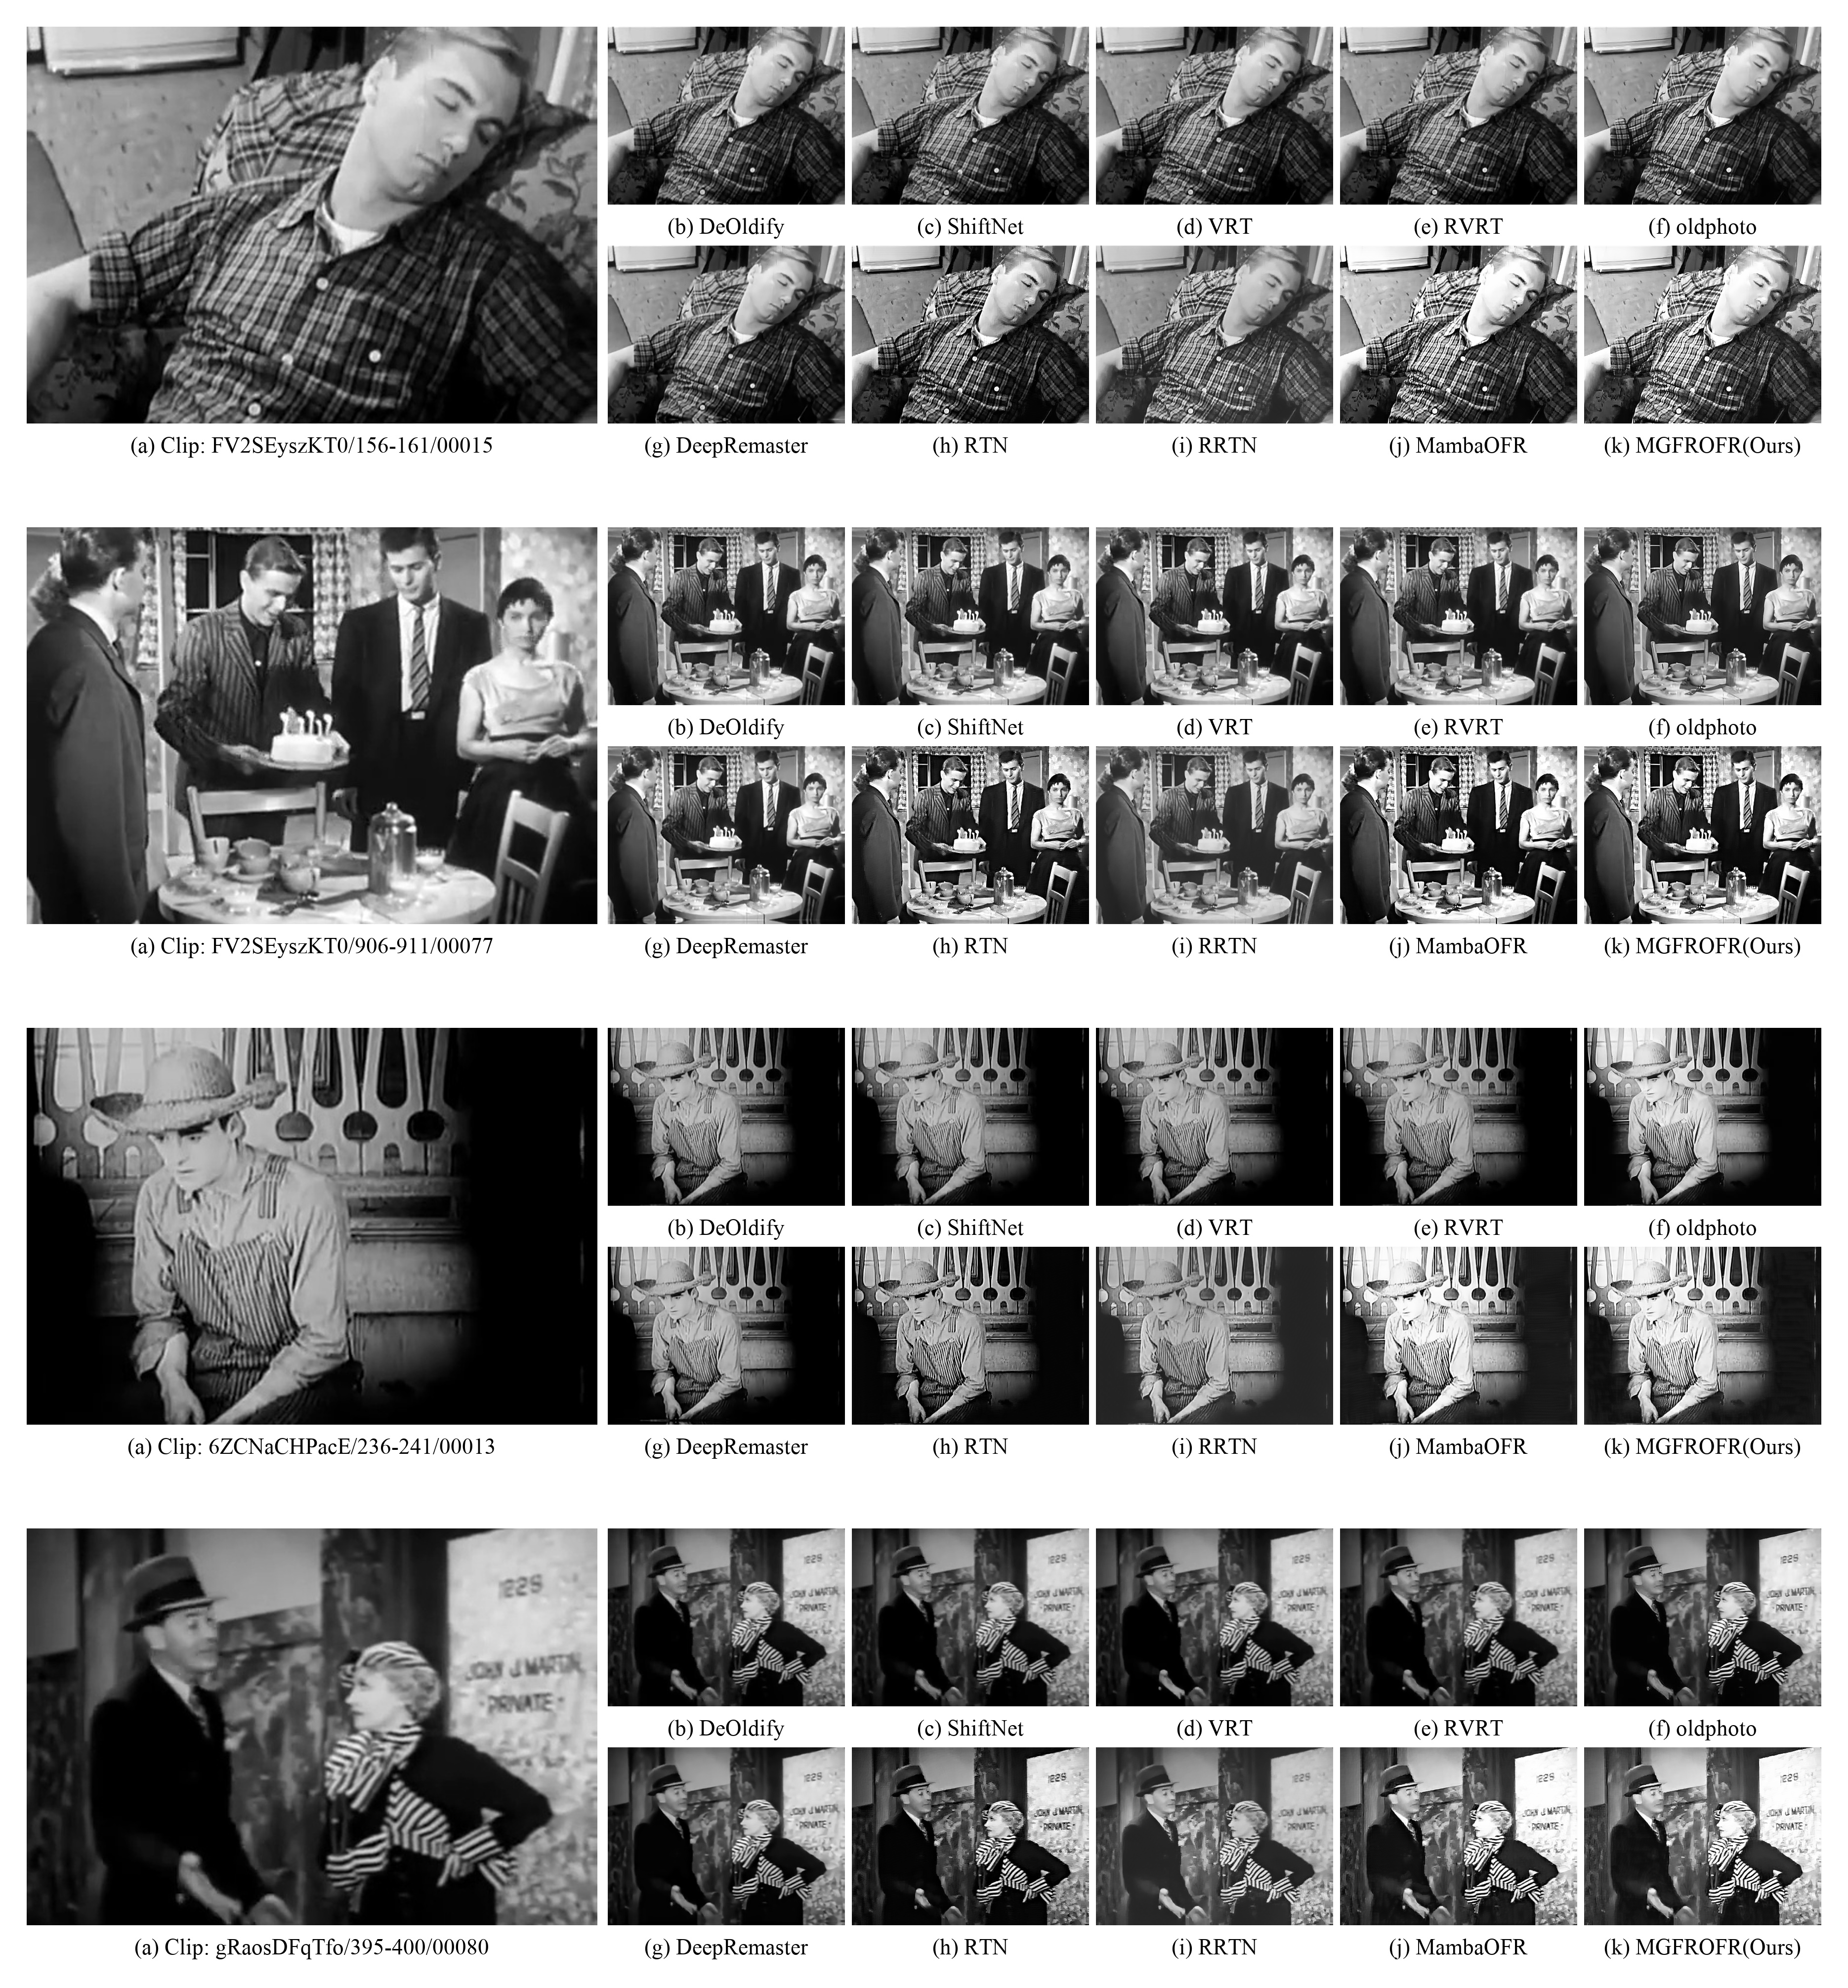
\includegraphics[width=0.95\textwidth]{figures/Fig5_SOTA_RealWorld_SRWOV_Qualitative.jpg}
\caption{Qualitative comparison on four representative SRWOV real-world clips. Each row shows one degraded input frame (a) and restoration results from DeOldify (b), ShiftNet (c), VRT (d), RVRT (e), OldPhoto (f), DeepRemaster (g), RTN (h), RRTN (i), MambaOFR (j), and MgfrOFR (Ours) (k). The selected clips cover facial close-ups, multi-person indoor scenes, strong vignetting, and high-contrast boundaries, illustrating that MgfrOFR suppresses residual old-film artifacts while preserving natural structure and local texture without relying on ground-truth references.\label{fig:qualitative_realworld}}
\end{figure}

Figure~\ref{fig:qualitative_realworld} compares visual results on four representative clips from the SRWOV real-world set: FV2SEyszKT0/\allowbreak 156--161/\allowbreak 00015, FV2SEyszKT0/\allowbreak 906--911/\allowbreak 00077, 6ZCNaCHPacE/\allowbreak 236--241/\allowbreak 00013, and gRaosDFqTfo/\allowbreak 395--400/\allowbreak 00080. Because no ground truth is available, the comparison focuses on visible artifact suppression, structural preservation, and naturalness. General video restoration methods reduce part of the photometric degradation but can leave residual scratches, stains, or contrast distortions. Image enhancement baselines may sharpen local texture while introducing over-enhancement around faces, clothing, and high-contrast boundaries. Compared with MambaOFR and the other OFR baselines, MgfrOFR more consistently preserves facial structure, fabric texture, object boundaries, and local contrast while suppressing residual old-film artifacts in these examples. These qualitative observations align with MgfrOFR's best NIQE and BRISQUE scores in Table~\ref{tab:realworld}; the CLIP-IQA+ ranking remains reported separately because it favors OldPhoto in the aggregate metric. MgfrOFR may still over-smooth very fine textures under extreme degradation, and severe motion blur can still cause flow-alignment errors; these cases are discussed in Section~\ref{subsec:failure}.



\FloatBarrier

\subsection{Ablation Study}
\label{subsec:ablation}

Table~\ref{tab:ablation} separates the effects of MGFE recalibration and RATR regularization. The setting names are kept consistent with Figure~\ref{fig:ablation_visual}. The +RATR only setting is a partial architectural control: MGFE branch descriptors are still computed as RATR ranking targets, while channel-wise recalibration is disabled.

\begin{table}[htbp]
\scriptsize
\caption{Ablation study on the SRWOV synthetic benchmark. The setting names match Figure~\ref{fig:ablation_visual}; ``MGFE''\ denotes channel-wise recalibration in this table. Best results are in \textbf{bold}.\label{tab:ablation}}
\centering
\begin{tabularx}{\textwidth}{>{\raggedright\arraybackslash}XccCCCC}
\toprule
\textbf{Setting} & \textbf{MGFE} & \textbf{RATR} & \textbf{PSNR$\uparrow$} & \textbf{SSIM$\uparrow$} & \textbf{LPIPS$\downarrow$} & \textbf{DISTS$\downarrow$} \\
\midrule
MambaOFR                        & Off & Off & 25.99 & 0.9059 & 0.0815 & 0.0822 \\
+MGFE only                 & On  & Off & 26.18 & 0.8960 & 0.1425 & 0.1132 \\
+RATR only                 & Off & On  & 26.84 & 0.9052 & 0.0963 & 0.0884 \\
MgfrOFR (Ours)             & On  & On  & \textbf{27.13} & \textbf{0.9237} & \textbf{0.0789} & \textbf{0.0653} \\
\bottomrule
\end{tabularx}
\end{table}

\noindent\textbf{Discussion.} MgfrOFR (Ours) improves MambaOFR by +1.14~dB in PSNR and achieves the best results across all four metrics. +MGFE only provides a small PSNR gain (+0.19~dB) but degrades LPIPS and DISTS, indicating that multi-granularity recalibration alone is insufficient. +RATR only gives a larger PSNR gain (+0.85~dB) and better perceptual balance. These results show that MGFE and RATR are complementary when used together.

\begin{figure}[htbp]
\centering
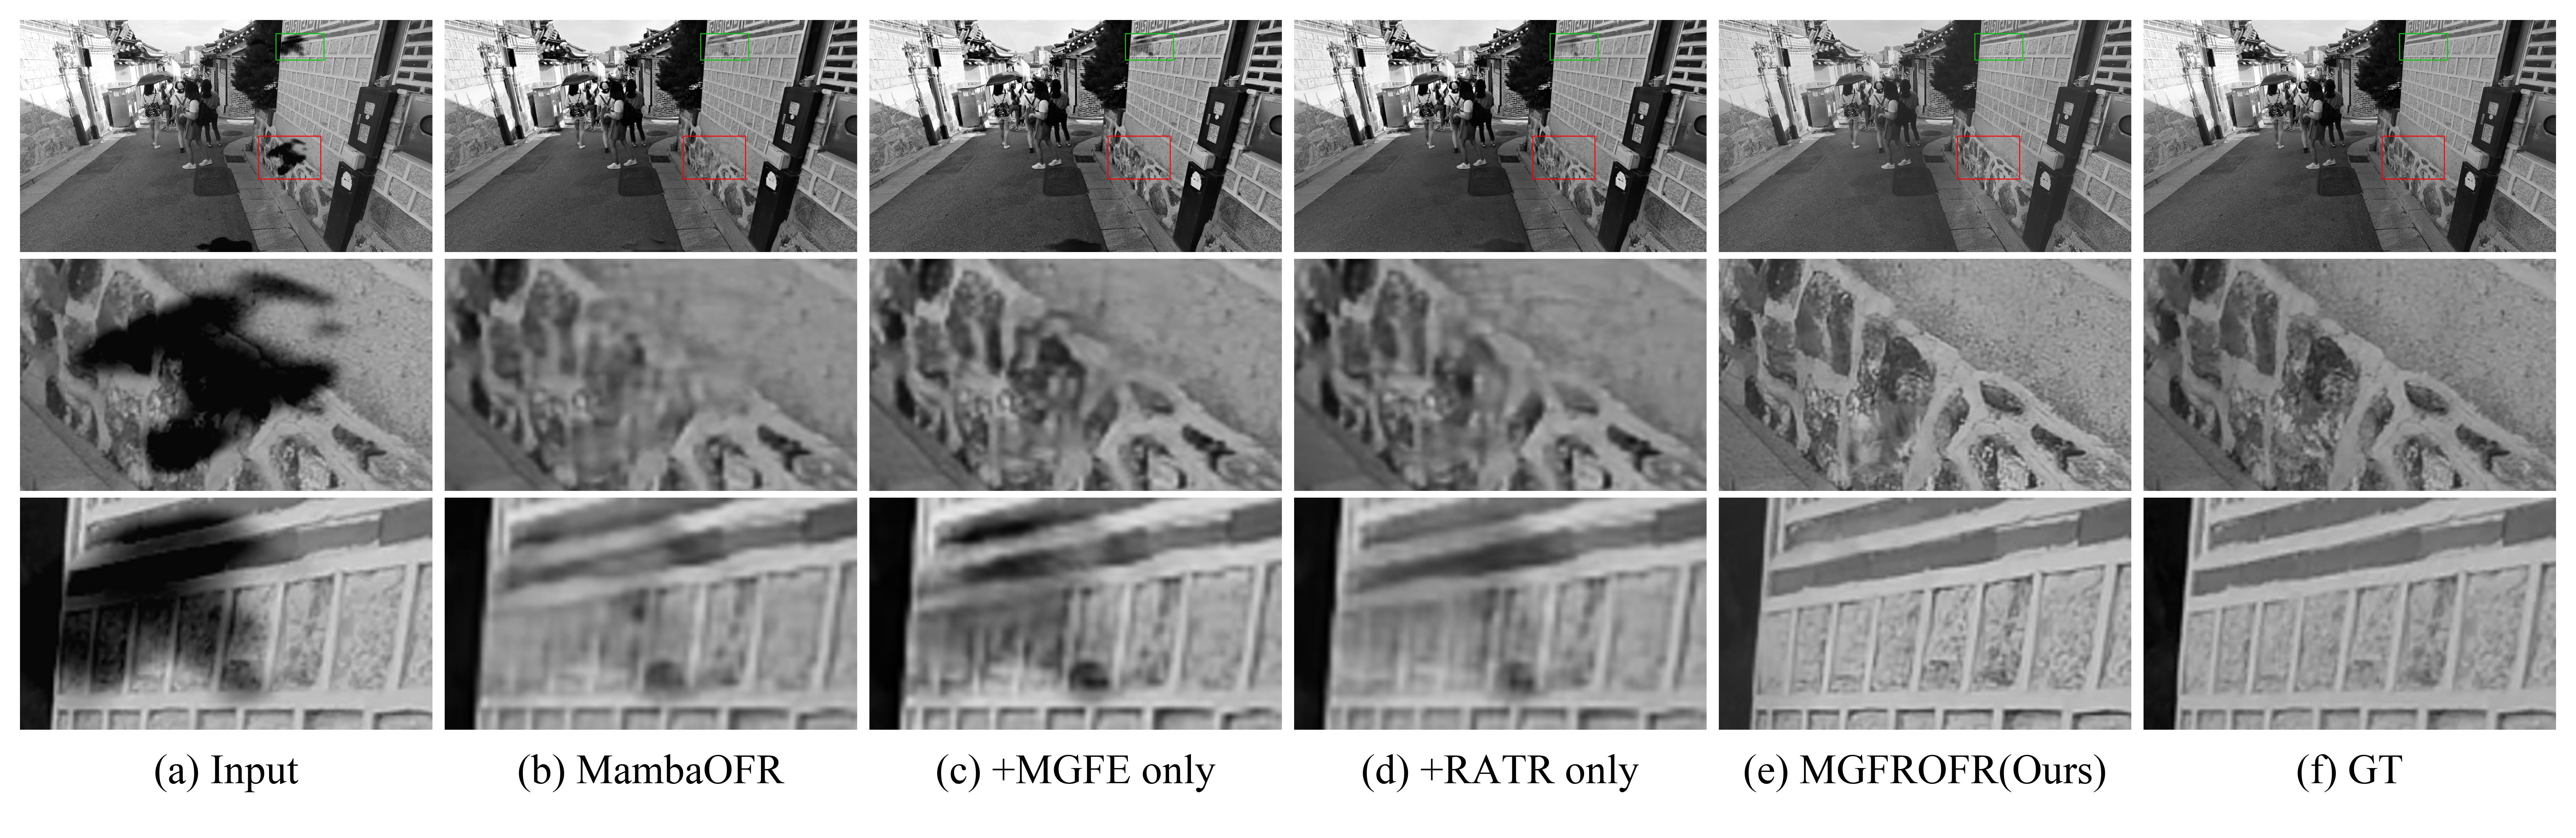
\includegraphics[width=0.95\textwidth]{figures/Fig6_Ablation_REDS_synthetic_Qualitative.jpg}
\caption{Visual ablation on REDS-based SRWOV synthetic data. \textbf{Top row:} full frames with red and green crop boxes marking the zoom regions. \textbf{Middle and bottom rows:} zoomed patches from the marked regions. From left to right, the restoration columns compare MambaOFR, +MGFE only, +RATR only, and MgfrOFR (Ours), with the degraded input and ground truth included as references. The comparison demonstrates that combining MGFE with RATR yields the cleanest local restoration among the ablated configurations in Table~\ref{tab:ablation}.\label{fig:ablation_visual}}
\end{figure}

\subsection{Hyperparameter Sensitivity}
\label{subsec:sensitivity}

We analyze MgfrOFR sensitivity to the main RATR and multi-granularity hyperparameters. Tables~\ref{tab:sensitivity_tau}--\ref{tab:sensitivity_granularity} report three groups: DKTau temperature $\tau$, RATR loss weights $\lambda_{\text{ratr}}$ and the intra/inter ratio, and the number of granularity branches $G$ and restoration tokens $M$. All experiments use the full MgfrOFR pipeline and are evaluated on the SRWOV synthetic benchmark.

\begin{figure}[H]
\centering
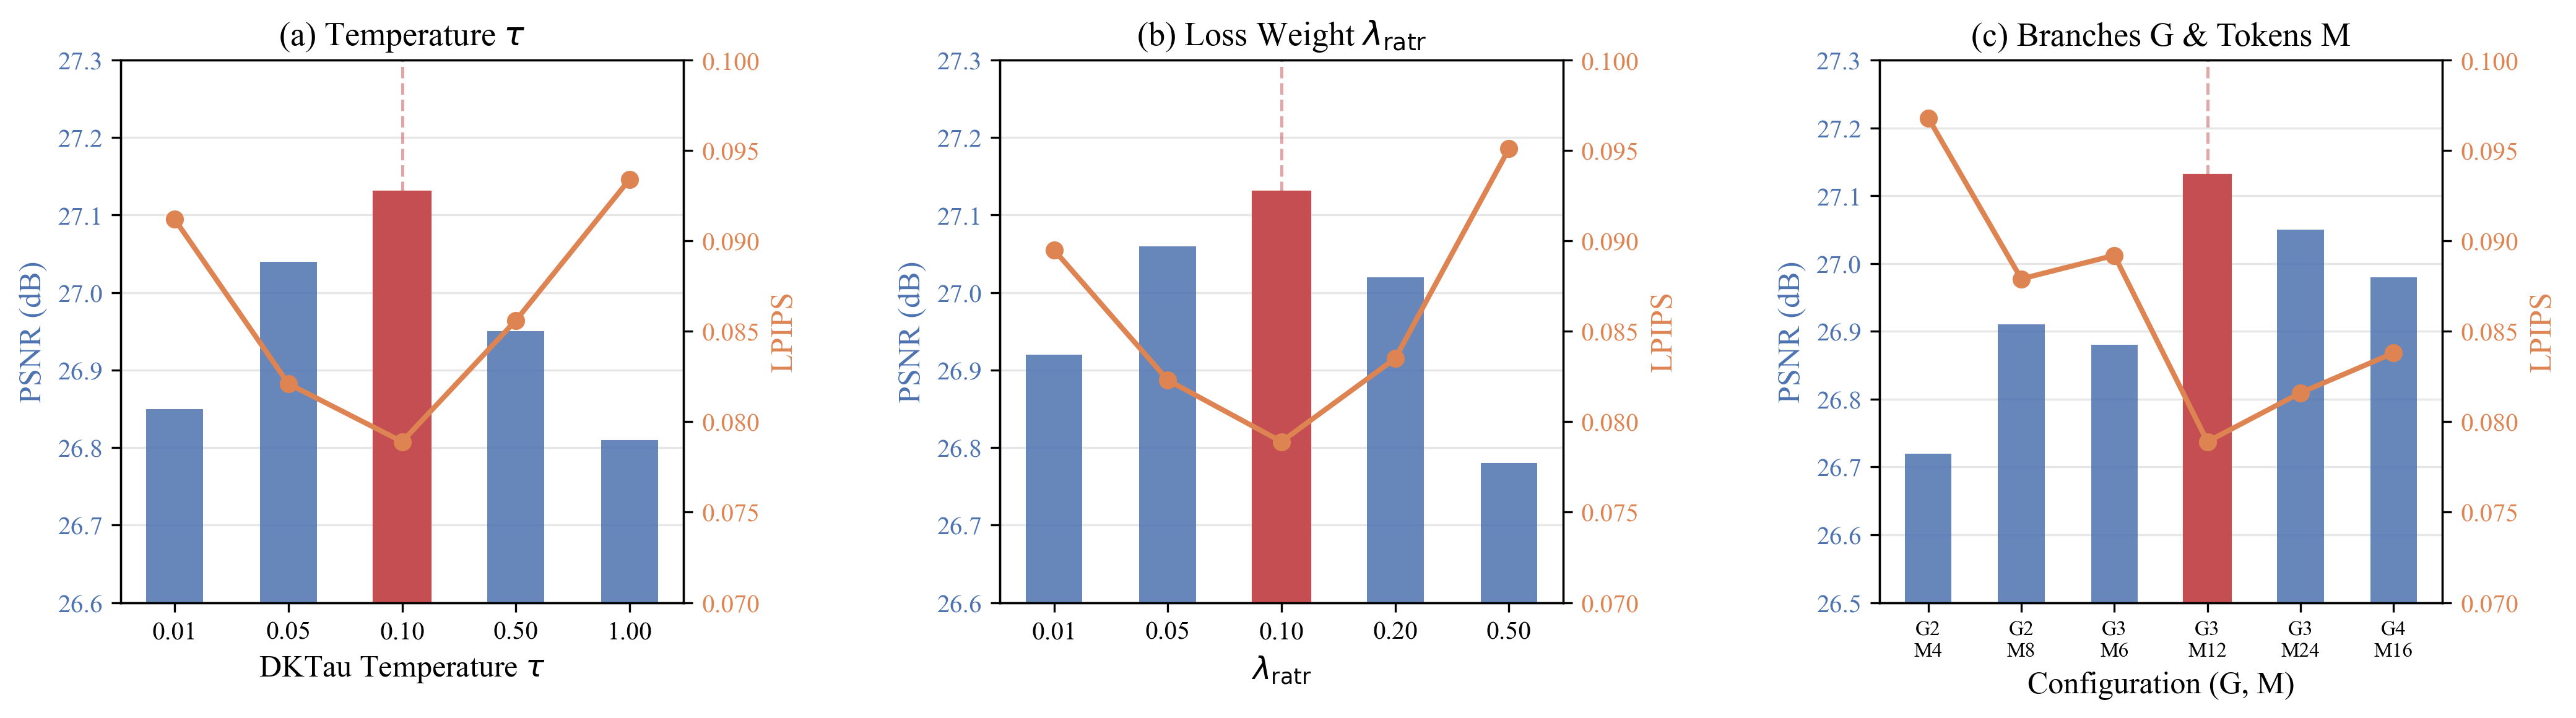
\includegraphics[width=0.95\textwidth]{figures/Fig7_sensitivity_analysis.png}
\caption{Hyperparameter sensitivity analysis. \textbf{Left:} DKTau temperature $\tau$. \textbf{Center:} RATR loss weight $\lambda_{\text{ratr}}$. \textbf{Right:} Number of branches $G$ and tokens $M$. The red bar (and the red dashed vertical line) marks the default configuration. PSNR is shown on the primary axis (bar); LPIPS on the secondary axis (line). The trends demonstrate that the default setting is a stable operating point rather than a brittle hyperparameter choice.\label{fig:sensitivity}}
\end{figure}

Figure~\ref{fig:sensitivity} summarizes the sensitivity trends across the three hyperparameter groups. Across the $\tau$ sweep, very small values make the ranking signal unstable, whereas overly large values oversmooth it. The RATR weight sweep follows the same pattern: weak regularization gives limited temporal constraint, while overly strong regularization reduces restoration flexibility. Together with the granularity sweep, these trends show that the default setting is a stable operating point within the tested range, without claiming global hyperparameter optimality.

\begin{table}[H]
\caption{Sensitivity to DKTau temperature $\tau$. The default setting is $\tau{=}0.1$.\label{tab:sensitivity_tau}}
\centering
\small
\begin{tabularx}{\textwidth}{CCCCC}
\toprule
$\tau$ & PSNR$\uparrow$ & SSIM$\uparrow$ & LPIPS$\downarrow$ & DISTS$\downarrow$ \\
\midrule
0.01  & 26.85 & 0.9068 & 0.0912 & 0.0871 \\
0.05  & 27.04 & 0.9121 & 0.0821 & 0.0825 \\
0.10  & \textbf{27.13} & \textbf{0.9237} & \textbf{0.0789} & \textbf{0.0653} \\
0.50  & 26.95 & 0.9098 & 0.0856 & 0.0843 \\
1.00  & 26.81 & 0.9054 & 0.0934 & 0.0878 \\
\bottomrule
\end{tabularx}
\end{table}

\begin{table}[H]
\caption{Sensitivity to RATR loss weights. Ratio denotes $\lambda_{\text{intra}}/\lambda_{\text{inter}}$; the default setting is $\lambda_{\text{ratr}}{=}0.1$ and ratio $2.0$.\label{tab:sensitivity_loss}}
\centering
\small
\begin{tabularx}{\textwidth}{ccCCCC}
\toprule
$\lambda_{\text{ratr}}$ & $\lambda_{\text{intra}}/\lambda_{\text{inter}}$ & PSNR$\uparrow$ & SSIM$\uparrow$ & LPIPS$\downarrow$ & DISTS$\downarrow$ \\
\midrule
0.01 & 2.0 & 26.92 & 0.9075 & 0.0895 & 0.0862 \\
0.05 & 2.0 & 27.06 & 0.9118 & 0.0823 & 0.0821 \\
0.10 & 2.0 & \textbf{27.13} & \textbf{0.9237} & \textbf{0.0789} & \textbf{0.0653} \\
0.20 & 2.0 & 27.02 & 0.9112 & 0.0835 & 0.0830 \\
0.50 & 2.0 & 26.78 & 0.9041 & 0.0951 & 0.0892 \\
\midrule
0.10 & 1.0 & 27.08 & 0.9125 & 0.0808 & 0.0815 \\
0.10 & 0.5 & 26.97 & 0.9095 & 0.0847 & 0.0839 \\
\bottomrule
\end{tabularx}
\end{table}

\begin{table}[H]
\caption{Sensitivity to the number of granularity branches $G$ and restoration tokens $M$. All configurations satisfy $M=k\cdot 2^{G-1}$; the default setting is $G{=}3$, $M{=}12$.\label{tab:sensitivity_granularity}}
\centering
\small
\begin{tabularx}{\textwidth}{ccCCCC}
\toprule
$G$ & $M$ & PSNR$\uparrow$ & SSIM$\uparrow$ & LPIPS$\downarrow$ & DISTS$\downarrow$ \\
\midrule
2 & 4   & 26.72 & 0.9032 & 0.0968 & 0.0895 \\
2 & 8   & 26.91 & 0.9082 & 0.0879 & 0.0856 \\
3 & 6   & 26.88 & 0.9070 & 0.0892 & 0.0864 \\
3 & 12  & \textbf{27.13} & \textbf{0.9237} & \textbf{0.0789} & \textbf{0.0653} \\
3 & 24  & 27.05 & 0.9115 & 0.0816 & 0.0822 \\
4 & 16  & 26.98 & 0.9101 & 0.0838 & 0.0835 \\
\bottomrule
\end{tabularx}
\end{table}

\FloatBarrier

\subsection{Complexity Analysis}
\label{subsec:complexity}

Table~\ref{tab:complexity} reports computational complexity under a unified measurement protocol in the same experimental environment described in Section~\ref{subsec:implementation}. Params/FLOPs for MambaOFR, MgfrOFR, and RTN are measured with PyTorch FlopCounterMode on a $1{\times}7{\times}3{\times}256{\times}256$ input, including the seven-frame forward pass and RAFT optical-flow front end. RRTN and DeepRemaster retain published Params/FLOPs because the released implementations are not directly compatible with this measurement path. Speed is reported as one mock training step divided by the seven frames in the clip.

\begin{table}[htbp]
\caption{Computational complexity comparison under the unified measurement protocol.\label{tab:complexity}}
\begin{tabularx}{\textwidth}{lCCCC}
\toprule
\textbf{Method} & \textbf{Params (M)} & \textbf{FLOPs (G)} & \textbf{Train Mem. (GB)$\downarrow$} & \textbf{Speed (ms/frame)$\downarrow$} \\
\midrule
DeepRemaster~\cite{iizuka2019deepremaster}  & 9.88  & 65.3   & 1.7   & 21.3  \\
RTN~\cite{wan2022rtn}                       & 6.18  & 2445.7 & 6.8   & 65.3  \\
RRTN~\cite{lin2024rrtn}                    & 7.54  & 3088.7 & 22.1  & 386.9 \\
MambaOFR~\cite{mao2025mambaofr}            & 3.49  & 2832.8 & 6.5   & 369.0 \\
\midrule
MgfrOFR (Ours)                              & 3.50  & 2846.9 & 7.0   & 396.9 \\
\bottomrule
\end{tabularx}
\end{table}

MgfrOFR adds 0.011M parameters (+0.32\%) and 14.1G FLOPs (+0.50\%) over MambaOFR. The added cost comes from restoration-token insertion, branch-specific token mixers in MGFE, and the training-only pairwise similarity computation in RATR. These additions keep MgfrOFR within the same computational order as MambaOFR while providing the restoration gains reported above.

\FloatBarrier

\subsection{Analysis and Limitations}
\label{subsec:analysis_limitations}

\subsubsection{Comparison with the Closest Prior Work}
\label{subsec:vs_mambaofr}

MgfrOFR is built directly on top of MambaOFR~\cite{mao2025mambaofr}, so its contribution should be distinguished from the baseline backbone. We do not claim originality for bidirectional Mamba propagation, the degradation-aware prompt block, or the original reconstruction head. The contribution of this work is the reorganization and regularization of propagated features before reconstruction.

Compared with MambaOFR, MgfrOFR differs in four implementation-level aspects. First, the propagated feature is no longer treated as a single restoration carrier; MGFE exposes explicit coarse-to-fine branches. Second, these branches are summarized and fed back through channel-wise recalibration rather than used only for auxiliary supervision. Third, branch diversity is constrained by ranking correlation on temporal correspondences rather than by an identity-based objective from recognition tasks. Fourth, RATR is used only during training, so the deployment interface remains compatible with the baseline inference pipeline.

The symmetry-related claim is limited to representation balance. MgfrOFR does not model object-level geometric regularity and does not propose a general mathematical theory of symmetry. Instead, it studies whether coarse-to-fine restoration branches can remain balanced under asymmetric film degradation. MGFE separates evidence by restoration granularity, and RATR discourages redundant temporal-similarity rankings across branches.

\subsubsection{MGFE--RATR Synergy for Branch Balance}
\label{subsec:synergy}

The ablation study indicates that MGFE and RATR have different roles in the full model. RATR alone provides a stronger and more stable gain than MGFE recalibration alone (Table~\ref{tab:ablation}) because the RATR-only configuration still computes MGFE branch descriptors and uses them as multi-granularity ranking targets; only the channel-wise scale/shift feedback is disabled. MGFE creates the branch structure needed for coarse-to-fine feature balance, whereas RATR makes the branches more complementary by suppressing redundant temporal-ranking behavior.

The real-world results are consistent with this interpretation but do not prove content fidelity without ground truth. On the SRWOV real-world test set (Table~\ref{tab:realworld}), MgfrOFR achieves the best NIQE and BRISQUE and remains competitive on CLIP-IQA+, suggesting that the multi-granularity decomposition transfers useful restoration structure beyond the synthetic training distribution. Because these are no-reference metrics, the claim is limited to statistical naturalness and metric-based perceptual quality.

\subsubsection{Branch Balance Analysis}
\label{subsec:branch_analysis}

The branch analysis assesses whether the granularity branches remain complementary rather than becoming correlated copies of the same descriptor. We compute pairwise cosine similarity between branch descriptors on the SRWOV synthetic test set. This analysis directly supports the representation-balance claim: useful branches should remain comparable but not redundant.

The full model yields lower inter-branch similarity than the MGFE-only variant (Figures~\ref{fig:branch_similarity} and~\ref{fig:branch_error_map}). This supports the role of RATR as the mechanism that keeps granularity branches functionally distinct. The RATR-only variant remains closer to the full model than to MGFE-only, which further indicates that ranking diversity regularization suppresses collapse even before recalibration feedback is enabled.

Figure~\ref{fig:branch_similarity} illustrates this contrast for a representative frame. In the MGFE-only configuration, the off-diagonal similarities remain high, indicating that the branches encode nearly the same restoration evidence. In the full model, these off-diagonal values decrease markedly, especially for the fine-grained branch, showing a more differentiated branch geometry.

\begin{figure}[!t]
\centering
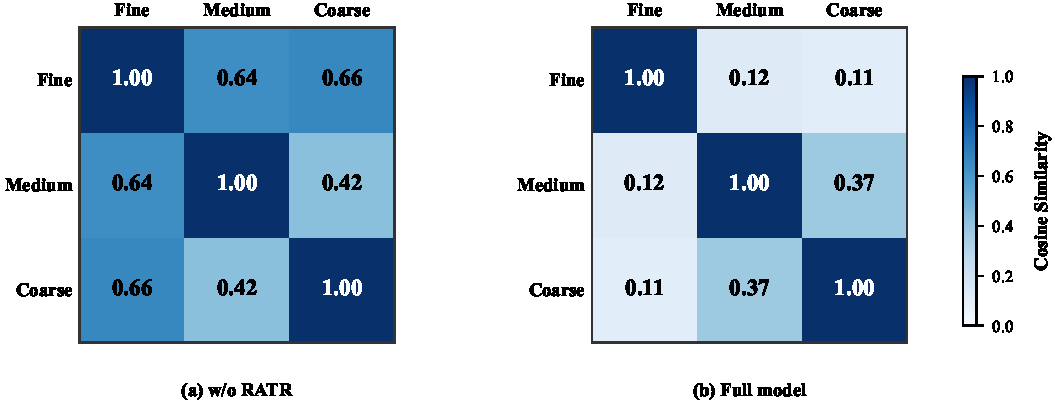
\includegraphics[width=0.84\textwidth]{figures/Fig9a_branch_similarity.pdf}
\caption{Branch balance analysis. Pairwise cosine similarity is compared between the MGFE-only configuration and the full MgfrOFR model. RATR reduces off-diagonal similarity from 0.42--0.66 to 0.11--0.37, confirming that ranking-aware regularization prevents granularity branches from collapsing into correlated descriptors.\label{fig:branch_similarity}}
\end{figure}

\begin{figure}[!t]
\centering
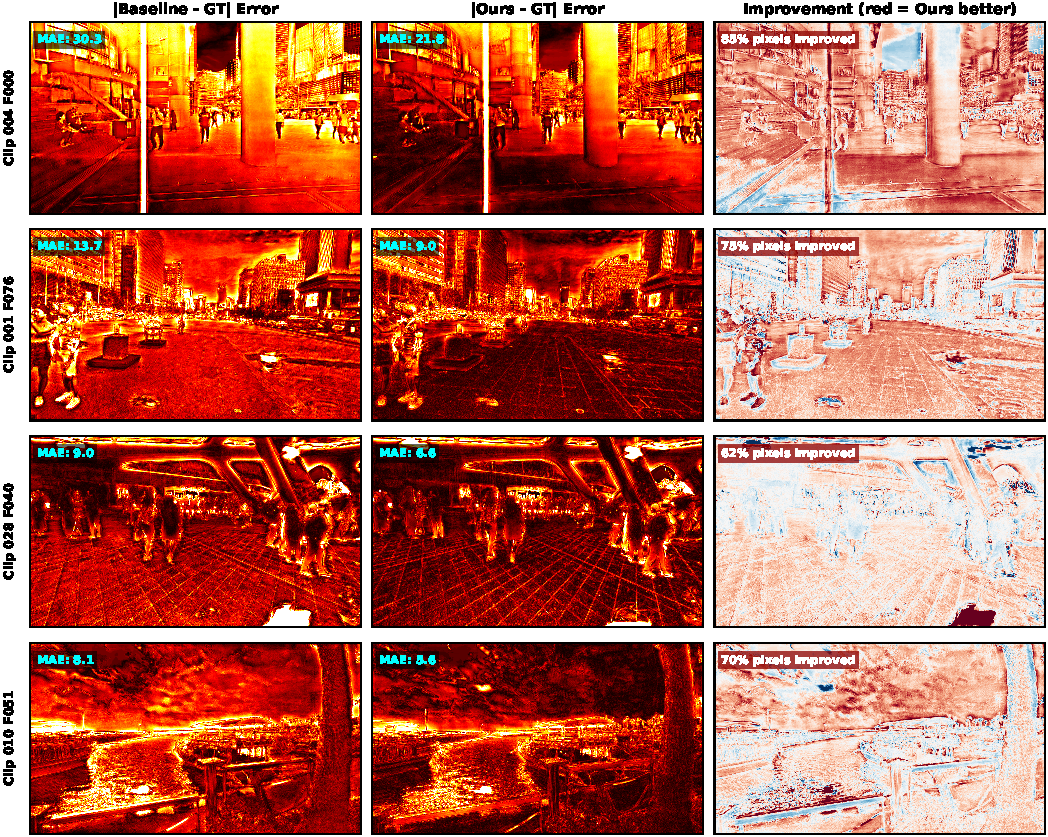
\includegraphics[width=0.98\textwidth]{figures/Fig9b_error_map.pdf}
\caption{Pixel-wise absolute-error comparison on four gate-selected synthetic frames. The left and middle columns compare $|$Baseline $-$ GT$|$ and $|$MgfrOFR $-$ GT$|$; the right column illustrates their difference, where red indicates regions in which MgfrOFR reduces the reconstruction error. The error maps demonstrate that lower branch correlation translates into spatially broader restoration gains rather than isolated local fixes.\label{fig:branch_error_map}}
\end{figure}

The inspected examples suggest a consistent specialization pattern. The fine-grained branch is most sensitive to localized defects such as scratches and pixel-level noise; the coarse branch emphasizes broader structural corruption such as blotches and cracks; and the medium branch occupies an intermediate role. This behavior is consistent with progressive token fusion, where fewer surviving tokens aggregate over wider spatial support. The pixel-domain error maps in Figure~\ref{fig:branch_error_map} further indicate that branch decorrelation corresponds to broader restoration gains rather than isolated local fixes.

\subsubsection{When Does MgfrOFR Struggle?}
\label{subsec:failure}

MgfrOFR's advantage is not uniform across all degradation conditions. The ablation study (Table~\ref{tab:ablation}) shows that MGFE alone degrades perceptual quality, and the visual ablations suggest that the full model is most useful when heterogeneous degradation is present, such as structural damage co-occurring with fine scratches in the same frame. On clips dominated by a single degradation type, such as uniform flicker without spatial damage, the multi-granularity decomposition can add representational overhead without proportional benefit, and the baseline or RATR-only variant may match the full model's fidelity.

The real-world CLIP-IQA+ result highlights a trade-off between naturalness and enhancement-oriented perceptual quality. MgfrOFR's CLIP-IQA+ (0.4368) ranks second to OldPhoto (0.4503), while MgfrOFR achieves the best NIQE (5.06) and BRISQUE (18.70). This pattern reflects that different no-reference metrics measure distinct aspects of restoration quality. CLIP-IQA+ is trained on human quality annotations that correlate with sharp textures and high-contrast details~\cite{wang2023clipiqa}, favoring methods such as OldPhoto that enhance perceptual sharpness through learned global priors. NIQE and BRISQUE instead measure statistical deviation from natural image distributions and penalize artifacts introduced by texture hallucination. MgfrOFR's granularity-based recalibration operates conservatively on the propagated feature stream, which appears to preserve statistical naturalness while providing less texture enhancement than OldPhoto. For archival restoration, NIQE/BRISQUE may be more relevant proxies when content fidelity is prioritized, but a human study is needed to validate that preference.

\subsubsection{Limitations, Threats to Validity, and Future Work}
\label{subsec:limitations}

\paragraph{Threats to Validity.}
Five threats affect the interpretation of the results. \textbf{Dataset threat}: all training uses synthetic degradation applied to REDS clips, which introduces a synthetic-to-real domain gap and may limit generalization to archival footage with correlated degradation chains not modeled by the pipeline. \textbf{Metric threat}: evaluation relies on PSNR/SSIM for pixel fidelity and no-reference metrics for real-world assessment; these metrics emphasize different aspects of quality and may not fully align with human perceptual judgments, especially for perceptual metrics where inter-clip variance prevents statistical significance at $N{=}30$. \textbf{Human-evaluation threat}: the study does not include an expert reader study with film-restoration practitioners or archivists, so the practical value of improvements on authentic footage is inferred from proxy metrics and qualitative inspection. \textbf{Baseline threat}: three baselines (VRT, RVRT, ShiftNet) required adaptation from video restoration to OFR-specific degradation, which preserves their architectures but may not reflect their optimal performance under a different training regime. \textbf{Synthetic-to-real threat}: the real-world evaluation lacks ground truth, so improvements in NIQE/BRISQUE reflect statistical naturalness rather than verified content fidelity, and the absence of external validation on additional datasets weakens the generalization claim.

\paragraph{Limitations and Future Work.}
RATR adds a training-time cost because it requires branch-wise similarity matrices over the batch-time descriptor set $\bar{N}=BT$. Its dominant cost therefore grows approximately quadratically in $\bar{N}$. In our setting ($B{=}4$, $T{=}7$, $G{=}3$), the total overhead of MGFE and RATR is 0.5\,GB (7.0 vs.\ 6.5\,GB; Table~\ref{tab:complexity}); however, longer clips or larger effective batch-time products would make this quadratic term more pronounced. Gradient checkpointing or selective ranking construction, such as sampling a subset of anchors per iteration, will be needed for larger training settings. The second limitation is the synthetic-to-real domain gap caused by REDS-based training degradation. Although the real-world NIQE/BRISQUE results are encouraging, authentic archival footage can contain correlated degradation chains that synthetic pipelines do not model. The third limitation is evaluation scope: validation is limited to SRWOV, and additional archival datasets plus human evaluation would strengthen the generalization claim.

Promising extensions include adaptive branch activation conditioned on degradation severity, frequency-aware branch specialization that assigns structural recovery and texture restoration to dedicated branches, and joint OFR--colorization frameworks for archival digitization and cultural heritage restoration workflows~\cite{kokaram2004missing}.

\section{Conclusions}
\label{sec:conclusion}

We presented MgfrOFR, a Mamba-based old film restoration framework that augments MambaOFR with explicit multi-granularity feature balancing. MGFE reorganizes propagated features into coarse-to-fine restoration-token branches and recalibrates the spatial stream through channel-wise feedback. RATR discourages branch collapse by penalizing correlated temporal-similarity rankings during training while preserving the baseline inference interface.

The SRWOV results support the claim that coarse-to-fine branch balance improves old film restoration under heterogeneous degradation. Under the unified reproduction protocol on the SRWOV synthetic benchmark, MgfrOFR achieves the strongest full-reference scores among the tested baselines, improving PSNR by 1.14~dB over MambaOFR (27.13~dB vs.\ 25.99~dB) with only 0.32\% additional parameters. On 216 real-world archival clips, MgfrOFR obtains the lowest NIQE and BRISQUE while remaining competitive on CLIP-IQA+. Because the real-world setting lacks ground truth, these no-reference gains should be interpreted as evidence of improved statistical naturalness rather than definitive proof of perceptual superiority. The ablation study further shows that MGFE and RATR are complementary: MGFE alone provides limited gains, whereas the full model improves fidelity and aggregate perceptual scores when branch diversity is explicitly enforced.

Several limitations define the scope of the conclusion. The method inherits the synthetic-to-real domain gap of REDS-based training; RATR adds a training-time cost that grows approximately quadratically with the batch-time descriptor set and increases training time by approximately 7.6\% over MambaOFR under our setting; and evaluation is limited to the SRWOV benchmark plus no-reference proxies on authentic footage. Future work will focus on adaptive branch activation conditioned on degradation severity, frequency-aware branch specialization that assigns structural recovery and texture restoration to dedicated branches, lighter ranking constructions such as selective anchor sampling, human-in-the-loop evaluation, and broader validation on additional archival benchmarks.


\vspace{6pt}

\authorcontributions{Conceptualization, F.C. and Y.D.; methodology, F.C.; software, F.C.; validation, F.C. and Q.Z.; formal analysis, F.C.; investigation, F.C.; resources, K.Y., L.C. and Y.D.; data curation, F.C.; writing---original draft preparation, F.C.; writing---review and editing, Q.Z., K.Y., L.C. and Y.D.; visualization, F.C.; supervision, Y.D.; project administration, Y.D.; funding acquisition, Y.D. All authors have read and agreed to the published version of the manuscript.}

\funding{This research received no external funding.}

\institutionalreview{Not applicable.}

\informedconsent{Not applicable.}

\supplementary{Not applicable.}

\dataavailability{The training data follow the public REDS benchmark and the SRWOV protocol described by MambaOFR. The manuscript source and figures are included in this submission package. Code, configurations, and evaluation scripts for this study are publicly available at \url{https://github.com/wscffaa/MgfrOFR}. Public benchmark data should be obtained from the original REDS and SRWOV/MambaOFR sources; no new dataset is redistributed in this work.}

\acknowledgments{The authors thank the developers of MambaOFR for releasing their code and pretrained models.}

\conflictsofinterest{The authors declare no conflicts of interest.}

\abbreviations{Abbreviations}{
The following abbreviations are used in this manuscript:
\par\smallskip
\noindent
\footnotesize
\begin{tabularx}{\textwidth}{@{}>{\raggedright\arraybackslash}p{0.2\textwidth}X@{}}
OFR & Old Film Restoration\\
MgfrOFR & Proposed old film restoration framework in this work\\
MGFE & Multi-Granularity Feature Extractor\\
RATR & Ranking-Aware Triplet Regularization\\
SSM & State Space Model\\
PSNR & Peak Signal-to-Noise Ratio\\
SSIM & Structural Similarity Index\\
LPIPS & Learned Perceptual Image Patch Similarity\\
DISTS & Deep Image Structure and Texture Similarity\\
NIQE & Natural Image Quality Evaluator\\
BRISQUE & Blind/Referenceless Image Spatial Quality Evaluator\\
CLIP-IQA+ & CLIP-based Image Quality Assessment (enhanced)\\
SRWOV & Synthetic + Real-World Old Video\\
REDS & REalistic and Diverse Scenes\\
GT & Ground Truth\\
CNN & Convolutional Neural Network\\
GPU & Graphics Processing Unit\\
\end{tabularx}
}

\begin{adjustwidth}{-\extralength}{0cm}
\reftitle{References}
\bibliography{references}
\PublishersNote{}
\end{adjustwidth}
\end{document}
